\chapter{XChange: Generic Asset Trading in Resource-constrained Environments}
\label{chapter:xchange}

\emph{An increasing number of industries rely on Internet-of-Things devices to track physical resources.
	Blockchain technology provides primitives to represent these resources as digital assets on a secure distributed ledger.
	Due to the proliferation of blockchain-based assets, there is an increasing need for a generic mechanism to trade assets between isolated platforms.
	To date, there is no such mechanism without reliance on a trusted third party. }
	
\emph{In this work, we address this shortcoming and present XChange.
	%Unlike existing approaches for decentralized asset trading, we decouple trade management and the actual exchange of assets.
	XChange mediates trade of \emph{any} digital asset between isolated blockchain platforms while limiting the fraud conducted by adversarial parties.
	We first describe a generic, five-phase trading protocol that establishes and executes trade between individuals.
	This protocol accounts full trade specifications on a separate blockchain.
	%We show with a theoretical analysis that the effectiveness of fraud conducted by adversarial parties is limited.
	We then devise a lightweight system architecture, composed of all required components for a generic asset marketplace.}
	
\emph{We implement XChange and conduct real-world experimentation.
	We leverage an existing, lightweight blockchain, TrustChain, to account all orders and full trade specifications.
	By deploying XChange on multiple low-resource devices, we show that a full trade completes within half a second.
	To quantify the scalability of our mechanism, we conduct further experiments on our compute cluster.
	We conclude that the throughput of XChange, in terms of trades per second, scales linearly with the system load.
	Furthermore, we find that XChange exhibits superior throughput and order fulfil latency compared to related decentralized exchanges, BitShares and Waves. }

\newpage

\section{Introduction}
Advancements in wireless technology, sensor networks, and hardware capabilities have resulted in exponential growth of low-resource devices operating within the Internet-of-Things (IoT)~\cite{makhdoom2018blockchain}.
%This is achieved by the deployment of numerous devices, often with low hardware capabilities, that communicate with each other.
IoT technology holds the potential to address societal challenges such as food security, sustainable agriculture, and renewable transportation~\cite{atzori2017understanding}.
Gartner estimates that by 2020, the Internet-of-Things consists of 20 billion Internet-connected devices worldwide~\cite{hung2017leading}.
%Internet-of-Things is said to be the breakthrough to enable a \enquote{smart society} and further espouses the digital transformation of many companies operating within industrial markets such as energy, healthcare and the automotive sector.

Many industries have deployed devices for the global traceability of assets, resources, or services.
%These devices keeps track of a \enquote{virtual biography} of the life of a specific asset.
For example, a smart meter installed at the home of a consumer keeps track of the energy usage of a specific household and reports these values to the energy provider.
Likewise, a GPS tracker installed in taxis calculates the traveled distance, so the driver knows how much to charge its passengers for a ride.
Such use-cases require an accountability mechanism to securely record the events that influence the state of an asset, e.g., physical movement or ownership change.

One of the solutions that can bring accountability features to the Internet-of-Things is blockchain technology.
Blockchain is a paradigm to create, manage and transfer digital assets in a tamper-proof manner.
This management is achieved by maintaining a distributed ledger that enables secure recording of transactions between digital entities, even within the context of mutual distrust.
The distributed ledger, also called a blockchain, is operated by network participants themselves without any dependency on trusted third parties.
From a business perspective, it fosters collaboration between companies since it provides the means to securely record interactions and share data. % that do not necessarily trust each other.
%Numerous companies acting within the sharing economy, health care and energy sector are researching how blockchain technology can digitalizes existing (often labor-intensive) business processes.

% Tokenization of physical assets and the impact of IoT and AI (https://www.eublockchainforum.eu/sites/default/files/research-paper/convergence_of_blockchain_ai_and_iot_academic_2.pdf)

Various industries are using a blockchain to keep track of assets within their domain.
Representing assets on a distributed blockchain is also called \emph{tokenization}~\cite{TokenizationOP}.
The introduction of the Bitcoin cryptocurrency and the popularity of blockchain technology in general have resulted in a proliferation of different types of digital assets, fragmented across many blockchain implementations.
Currently, almost 200.000 different assets are being managed on the Ethereum blockchain only.\footnote{https://etherscan.io/tokens} % implemented only on the Ethereum blockchain.
While there is an abundance of different types of digital assets, there is no generic mechanism to exchange (trade) these assets between isolated blockchain platforms without the involvement of a trusted third party.
We argue that such a mechanism is a growing necessity, as more industries are relying on blockchain technology and tokenization of their resources.

%\begin{figure}[t]
%	\centering
%	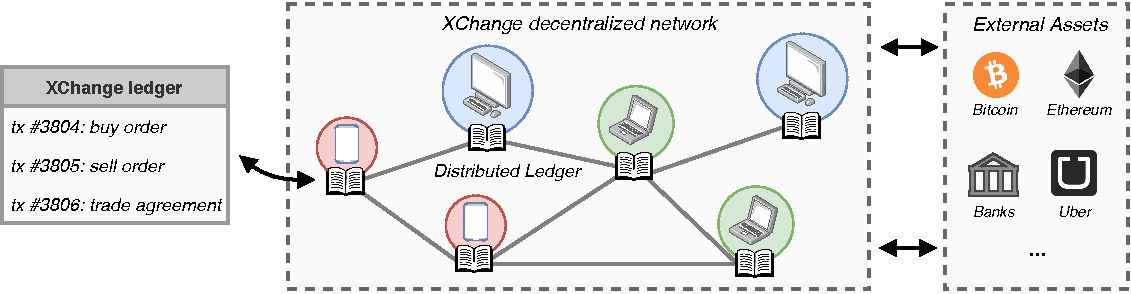
\includegraphics[width=\linewidth]{assets/idea}
%	\caption{A visualization of \ModelName{}, a blockchain-based mechanism for generic asset trading. The network maintain a distributed ledger that stores all market activity such as orders and trades. To exchange assets, peers communicate with external platforms such as Bitcoin, Ethereum or banks.}
%	\label{fig:idea}
%\end{figure}

We present \emph{\ModelName{}}, a blockchain-based mechanism for generic asset trading in resource-constrained environments.
In stark contrast to existing approaches, \ModelName{} enables the exchange of digital assets between practically \emph{any} blockchain platform without need for trusted third parties that mediate between market participants.
%\ModelName{} stores assets of the same type in wallets and mediates the trade between wallets in a lightweight manner.
\ModelName{} is highly applicable in situations where many different assets have to be managed and exchanged.
These situations include peer-to-peer energy trading, supply chain management, and service exchange within the sharing economy.

The key idea of \ModelName{} is to account full trade specifications on a blockchain.
%This includes all orders created by traders, and details on payments performed during a trade between two parties.
This accounting enables traders to accurately track the progress of ongoing trades.
A trade in \ModelName{} is modelled as a sequence of unilateral payments (asset transfers) between two trading parties.
\ModelName{} prevents a trader from initiating a trade with someone that currently have an obligation to initiate a payment to another trader during an ongoing trade.
This addresses the situation where an adversarial party steals assets by refusing to initiate a payment back to some counterparty after having received some assets.
As a result, an adversary can only commit this kind of fraud once.
To further reduce the gains of adversarial parties, \ModelName{} allows that each trade is divided in multiple payments.
We call this mechanism \emph{incremental settlement}.

%The fundamental design principle of \ModelName{} is to \emph{decouple trade management and the exchange of assets between traders}.
%The key design principle of \ModelName{} is to \emph{decouple order management and asset management}.
%Our approach is visualized in Figure~\ref{fig:idea} and originates from the observation that existing blockchain-based marketplaces for asset trading utilize the same underlying data structure to manage trade and to exchange assets.\todo{remove/rewrite?}
%Therefore, trade management is subject to the same security requirements as the exchange of assets between trading parties.
%By decoupling these two practices, we increase overall market throughput, since trade management requires different (lower) security guarantees than the exchange of assets.
%Peers in the \ModelName{} network maintain a distributed ledger that stores all orders and trade activity.
%These peers interact with external platforms to transfer assets to other traders.
%To store market activity , we build on a scalable blockchain ledger that is optimised for data accounting.
%By accounting full trade specifications, we show that the effectiveness of fraud conducted by adversarial parties is limited.

The main contribution of this work is five-fold:
\begin{enumerate}
	\item The \ModelName{} \emph{trading protocol} which specifies how cross-chain trade between two parties proceeds, and how fraud conducted by adversaries is limited. (Section \ref{sec:protocol}). %The protocol is compatible with any type of distributed ledger that supports tamper-proof storage of data items.
	\item A lightweight \emph{system architecture} for generic, cross-chain trade (Section \ref{sec:architecture}).
	%\item Anti-fraud measures through full accounting of trade records, such that the effectiveness of fraud conducted by adversarial parties is limited (Section \ref{sec:security}).
	\item An improvement of TrustChain \cite{otte2017trustchain}, the consensus-less blockchain solution used by \ModelName{}, that enables concurrent transactions and increases scalability (Section~\ref{sec:blockchain_accounting}).
	\item A fully functional, open source \emph{implementation} of the \ModelName{} trading protocol and system architecture (Section \ref{sec:implementation}).
	\item \emph{Experimentation} around the resource usage and scalability of \ModelName{}, conducted on multiple low-resource devices and our compute cluster (Section~\ref{sec:exp_trading_low_devices}, \ref{subsec:scalability_experiment} and \ref{sec:experiment_comparison}).
\end{enumerate}

\section{Background and Problem Description}
This work focuses on how to trade digital assets that are stored on different blockchains, without the need for a trusted market operator that mediates in the trading process.
We first provide background on electronic marketplaces and elaborate how blockchain technology enables decentralized asset marketplaces.
We then formulate the problem description and pose the cardinal research question that this work answers.
%For brevity reasons, we assume that asset trading also encompasses the exchange of resource and services since they can be interpreted (tokenized) as digital assets.

\subsection{Electronic Marketplaces}
For decades, the ability to facilitate trading at a global scale has been at the core of many established companies operating on the Internet.
In 1995, Craigslist already offered an unmoderated mailing list where strangers could negotiate, meet, and trade physical goods.
eBay formalized the concept of online trading by introducing a reputation system where buyers and sellers rate each other.
More recently, leading companies acting within the sharing economy, deployed global marketplaces for ride-hailing (Uber), accommodation (AirBnb), freelance labour (TaskRabbit), and many other services.
%We argue that decentralization is the next step, the ability to establish trade without the need for any trusted market operator.

The primary responsibility of electronic marketplaces is two-fold.
First, market operators have to ensure a quick and effective mediation between supply and demand.
In most electronic marketplaces, participants create supply and demand by submitting \emph{orders} to the market operator.
In general, literature distinguishes between two types of orders: \emph{offers} that indicate the willingness of traders to sell specific assets, and \emph{requests}, created by a party interested in specific assets.
Electronic marketplaces aggregate submitted offers and requests, and match them, based on their specifications.
This process is also called \emph{order matchmaking}.
%Specifically, traders that want to buy or sell assets submit orders to the platform to specify their intentions.
The second responsibility of electronic marketplaces is to execute trade between traders, as soon as a matching between an offer and a request is found.
The market operator either owns the items subject to trade (e.g., in forex markets), or acts as arbitrator in case of a dispute (e.g. AirBnb).
%However, in some electronic marketplaces, the platform is merely responsible for connecting traders together.

\subsection{Centralized Marketplaces}
To date, most electronic marketplaces are operated by a single market owner, responsible for defining and controlling the environment in which trade is executed~\cite{yarom2004decentralized}.
While it is a common practice to deploy marketplaces with a centralized authority and system architecture, it leads to a few deficiencies in general.
%First, reputation accumulated by traders is often locked to a single platform and cannot easily be transferred elsewhere.
%This results in fragmentation of one's trading history and makes it harder to estimate trustworthiness of other traders.
The first problem is that centralized systems tend to be less resistant against infrastructure failures and targeted attacks (e.g., a denial-of-service attack~\cite{mirkovic2004internet}).
Since digital assets are often stored on a single or a few servers, they pose an interesting target for attackers.
Second, the deployed business logic of (commercial) market operators is rarely open for inspection by traders.
The lack of audibility motivates market owners to exploit their prominent position.
For example, it is suspected that Uber manipulates ride prices with a dynamic pricing mechanism~\cite{chen2015peeking}.

The emergence of cryptocurrency exchanges, facilitating the trade of blockchain-based assets, further highlights issues underlying marketplaces under central control~\cite{moore2013beware}.
While a few of these exchanges process transactions worth millions of dollars in total daily, many market operators lack the knowledge or resources to quickly scale up their infrastructure to meet increasing demand.
More than once, the fragile infrastructure of centralized cryptocurrency exchanges has resulted in poor trading experiences, prolonged platform unavailability, and even the inability to withdraw assets from digital wallets by users~\cite{centralizedexchanges}.
The events surrounding the Mt. Gox cryptocurrency exchange in 2014, where hackers compromised Bitcoin worth around \$450 million, demonstrates that inadequate security measures can lead to irreversible reputational damage.

\subsection{Decentralized Marketplaces}
The shortcomings of centralized marketplaces motivate the deployment of blockchain-powered decentralized markets, or \emph{DEXes}.
On these DEXes, users can issue, manage and trade digital assets that are stored on a blockchain.
Furthermore, traders remain in full control of their assets, instead of having them managed by a single market operator.
DEXes leverage blockchain technology to transfer ownership of different types of assets at the same time, without the risk of these assets being compromised by an adversarial party.
Notable DEXes include Waves and BitShares, which obtained a market capitalization of \$80 million and \$83 million respectively at the time of writing~\cite{wavesplatform}~\cite{schuh2015bitshares}.
To date, there are more than 250 DEXes and over than 4.000 active traders across all DEXes~\cite{han2019optionality}.

A common characteristic of DEXes is that all orders created by traders are stored and processed on a blockchain.
To match compatible offers and requests, DEXes either execute matchmaking logic during transaction validation or they rely on a centralized server to conduct order matchmaking.
Although the market volume of DEXes is increasing, a DEX is limited to facilitate the trade of assets that are stored on its underlying blockchain.

%Compared to centralized market infrastructures, DEXes are more robustness against large-scale efforts to compromise assets, since wallets are not stored in a single location.
%However, decentralized market infrastructures introduce new problems.
%These problems include fraud management, dispute resolution, decentralized reputation management, and effective dissemination of market information.
%However, the performance (transaction throughput) of DEXes is often low due to the security requirements when managing digital assets.

\subsection{Asset Trading Between Different Blockchains}
Centralized cryptocurrency exchanges are able to trade assets stored on different blockchains through intermediate wallets owned by the market operator.
However, there are increasing trust issues around the companies operating these cryptocurrency exchanges~\cite{chohan2018problems}.
Although DEXes enable trust-less asset exchange without trusted third party, the trading is limited to assets managed on the blockchain used by a specific DEX.
The exchange of digital assets residing in two different blockchain platforms, e.g., exchanging Bitcoin and Ethereum assets, is a non-trivial problem.

The \emph{atomic swap} protocol addresses the problem of exchanging assets between different blockchains, without need for a trusted third party~\cite{herlihy2018atomic}.
Atomic swaps enable two parties to exchange blockchain-based assets in an atomic manner: the asset exchange either succeeds or fails for both parties at any given time.
The key technology underlying the atomic swap protocol is the Hashed Time-locked Contract, or HTLC~\cite{bowe2018hashed}.
This is a special type of blockchain transaction where a party must provide a pre-image of a cryptographic hash before some deadline, usually 24 hours, in order to claim his or her assets.
If this deadline is exceeded and a party did not provide the pre-image, the assets go back to the original owner.
Atomic swaps eliminate the \emph{counterparty risk} of losing assets to an adversarial trader while trading.
Counterparty risk is a serious concern in many electronic marketplaces that facilitate peer-to-peer trading~\cite{peters2016understanding}.

Although atomic swaps enable risk-free and cross-chain trading, we identify two deficiencies.
%We argue that atomic swaps are not a generic solution for trading assets between blockchain, for the following two reasons.
First, atomic swaps only work when trading assets between blockchains with support for specific programming constructs.
An atomic swap involving a blockchain platform without support for HTLCs is not possible.
Second, the atomic swap protocol is complicated to implement, and a single implementation mistake can result in the loss of funds.
We aim for a generic, cross-chain trading solution that does not rely on the availability of specialized transaction types.

\subsection{Problem Description}
\label{sec:problem_description}
%Most decentralized marketplaces address the problems inherent to decentralization using a blockchain ledger~\cite{subramanian2017decentralized}.
%Exchanges that are powered by blockchain technology are also called \emph{DEXes}.


%One might believe that atomic swaps are a solution to enable generic trade between different blockchain ledgers~\cite{herlihy2018atomic}.
%Atomic swaps are a technique to trade assets between two different blockchain implementations.
%The atomic swap is a recent innovation that allows two users to trade blockchain-based assets, e.g., Bitcoin and Ethereum, without the risk that any of the involved parties loses their assets to the counterparty.
%This risk is also called \emph{counterparty risk} and is a severe concern in many electronic marketplaces that allow for peer-to-peer trading~\cite{peters2016understanding}.
%The atomic swap process is cryptographically secured and does not involve any trusted third party.

%The second issue is that atomic swaps is not a mature technology yet.
%There are still various open attacks, e.g., the situation where a party that is currently involved in an atomic swap gets compromised.

In this work, we address the challenging problem of generic trade of digital assets between different blockchain platforms.
Due to the proliferation of blockchain-based assets, we believe that the availability of such a trading mechanism is becoming a necessity.
Based on the aforementioned deficiencies of existing centralized and decentralized marketplaces, we formulate three requirements for our cross-chain trading mechanism:

\begin{enumerate}
	\item \textbf{Generic}. We require that our trading mechanism enables generic trade of assets between different blockchain platforms. In particular, the trade of assets with our mechanism should not be limited to a selected number of blockchain architectures with specific design requirements. We do not consider the atomic swap protocol an adequate solution for such a trading mechanism since it requires support for HTLCs.
	\item \textbf{Decentralized}. We require that the architecture of our trading mechanism is decentralized, and that users themselves remain in control of the assets involved in a trade. More specifically, decentralization in the context of this work is achieved when there is not a single authority that controls the environment in which order matchmaking and trade execution take place. Trade should emerge and proceed through direct information exchange between traders and peer-to-peer payments.
	\item \textbf{Limited counterparty risk}. During a trade, a counterparty might actively try to fraud the other party for economic benefit. In centralized marketplaces, counterparty risk is usually addressed by the (trusted) market operator which mediates the asset exchange between two parties. In decentralized marketplaces, counterparty risk is reduced since blockchain technology allows a trust-less transfer of assets. Our solution requires adequate measures to limit counterparty risk while trading.
\end{enumerate}

These requirements directly lead to the following research question: \emph{how can we devise a generic and decentralized mechanism to trade assets that are stored on different blockchains, with limited counterparty risk?}

\section{Solution Outline}
In this section, we outline our solution for generic, cross-chain asset trading.
During the following example, we assume that two traders, Alice and Bob, exchange blockchain-based assets.
Prior to the actual asset exchange, they have signed a contractual agreement containing all details of the upcoming trade.
These details include the negotiated exchange price and wallet addresses, and is further explained in Section~\ref{sec:protocol}.
The trade agreement between Alice and Bob is public and can be inspected by anyone.
Assume that Alice wants to sell her Bitcoin (BTC) to Bob, in return for some of his Ethereum gas (ETH).
A peer-to-peer asset exchange involves at least a transfer of BTC assets from the Bitcoin wallet of Alice to the Bitcoin wallet of Bob, and a transfer of ETH assets from the Ethereum wallet of Bob to the Ethereum wallet of Alice.

\begin{figure}[t]
	\centering
	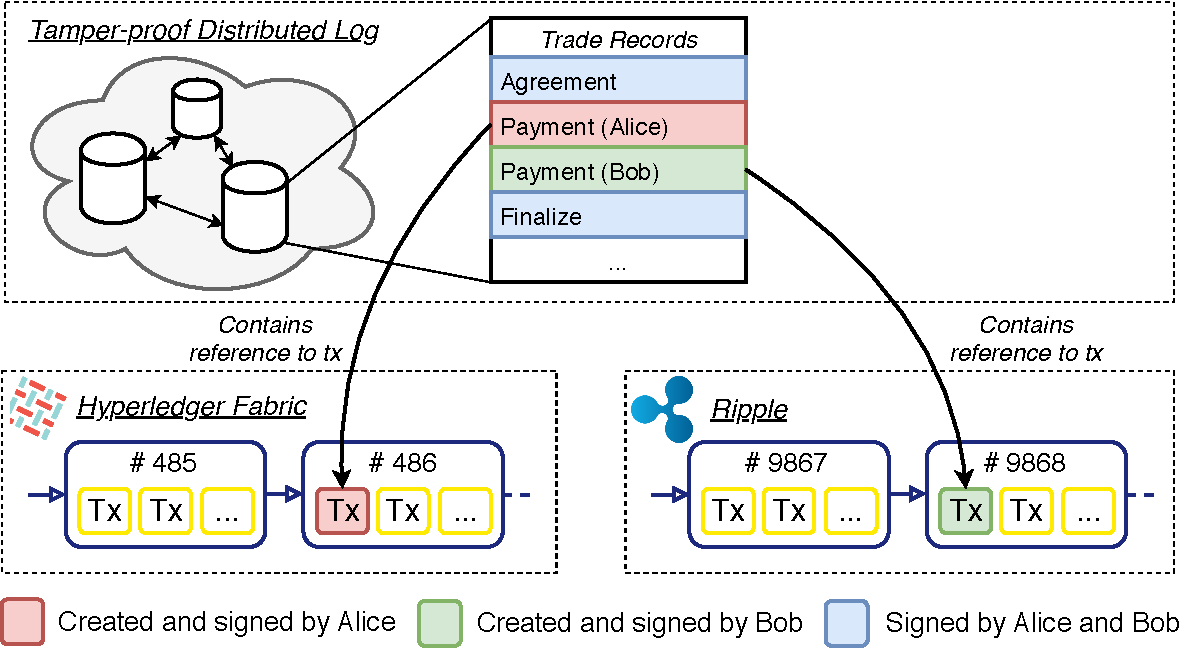
\includegraphics[width=.9\linewidth]{xchange/assets/xchange}
	\caption{High-level overview of our \ModelName{} trading mechanism. In this example, Alice trades her Bitcoin for Bob's Ethereum tokens. Full trade specifications are stored on a separate blockchain.}
	\label{fig:xchange}
\end{figure}

\subsection{Naive Approach}
We first consider a naive approach to trade the BTC and ETH assets between Alice and Bob, without any trusted third party.
W.l.o.g., we assume that Alice initiates the trading process and has to initiate the trade by sending assets to Bob.
She does so by submitting a transaction to the Bitcoin blockchain which transfers BTC assets from her Bitcoin wallet to the Bitcoin wallet of Bob.
When this transaction is included on the blockchain, she notifies Bob about the conducted payment.
As soon as Bob verifies that the BTC arrived his Bitcoin wallet, he initiates a transfer of ETH from his Ethereum wallet to the Ethereum wallet of Alice.
Both these asset transfers are included as individual transactions in the Bitcoin and Ethereum blockchains, and are publicly visible to other interested parties.
%These transactions are publicly accessible, embedded in both the Bitcoin and Ethereum ledger.
Therefore, others can verify that all assets have been transferred between Alice and Bob and that both parties fulfilled all obligations as specified in the trade agreement.
The exchange of assets during a trade is also called \emph{settlement}.

A major problem with this trade procedure, however, is that Bob can commit \emph{counterparty fraud} by simply refusing to transfer his ETH to Alice as soon as Alice has transferred her BTC to him.
Likewise, if Bob would initiate the first payment to Alice, Bob is exposed to the counterparty risk of losing his ETH to Alice.
Centralized exchanges usually address this counterparty risk by active mediation during an asset exchange between two parties.
In this situation, both Alice and Bob transfer their BTC and ETH respectively to wallets owned by the market operator.
The market operator then transfers the BTC assets to the Bitcoin wallet of Bob and the ETH assets to the Ethereum wallet of Alice.

\subsection{Our Solution}
This work aims to limit counterparty risk during the asset exchange process by relying on \emph{accountability}.
The key idea of our trading mechanism, called \emph{\ModelName{}}, is to store full specifications of each trade on a separate blockchain.
Our approach is visualized in Figure~\ref{fig:xchange}, which shows (parts of) the Bitcoin and Ethereum blockchain in the lower part of the figure, and the separate blockchain used by \emph{\ModelName{}} in the upper part of the figure.
Technical requirements of the \ModelName{} blockchain are discussed in Section~\ref{sec:blockchain_accounting}, and for now we assume that this blockchain is capable of storing arbitrary data elements in a secure manner.

The trade between Alice and Bob now proceeds as follows: first, one of the parties publishes the dual-signed trade agreement on the \ModelName{} blockchain (in Figure~\ref{fig:xchange}, this agreement is included in the block with sequence number 68.356).
%The trade between Alice and Bob now proceeds as follows: both Alice and Bob create an offer and request respectively, and include it within a transaction on the \ModelName{} blockchain.
%These offers indicate their interest in selling and buying some assets, and are indicated as a red and green transaction respectively in Figure~\ref{fig:xchange}.
%We assume that the created offer and request match, and the creators behind these orders are willing to trade with each other.\footnote{In our trading mechanism, \emph{matchmakers} bring potential traders together. This is further discussed in Section~\ref{sec:protocol}.}
%Alice and Bob now communicate with each other to create and sign a trade agreement, which is then included by one of the parties within a transaction on the \ModelName{} blockchain.
%This trade agreement is irrefutable and commits the involved traders to the upcoming trade. %, and is stored on the \ModelName{} blockchain within a single transaction by one of the parties.
Next, the settlement process starts, and Alice and Bob initiate payments to each other.
W.l.o.g., assume Alice starts the trade by initiating a transaction to send her BTC to the Bitcoin wallet of Bob.
In Figure~\ref{fig:xchange}, this transaction is included in the block with sequence number 486 on the Bitcoin blockchain.
Next, Alice records this payment within a transaction on the \ModelName{} blockchain, which includes the identifier of the transfer transaction on the Bitcoin blockchain.
When Bob wants to verify that Alice has indeed transferred the BTC to his Bitcoin wallet, he can inspect the BTC transaction and check it for validity and finality.
When Bob has confirmed that Alice indeed sent the BTC to his Bitcoin wallet, he initiates a payment to Alice by submitting a transaction to the Ethereum blockchain.
In Figure~\ref{fig:xchange}, this transaction is included in the block with sequence number 9.868 on the Ethereum blockchain.
Next, Bob records this payment within a transaction on the \ModelName{} blockchain.
Alice now verifies whether Bob has sent the promised ETH assets to her Ethereum wallet.
If so, both parties explicitly publish a transaction on the \ModelName{} blockchain (e.g. block 68359 in Figure~\ref{fig:xchange}) to indicate that the trade has completed successfully.

Note that the above solution requires that the assets subjected to a trade can be publicly traced.
We believe this is not a major limitation since ownership change of a vast majority of blockchain-based assets is public information.
Furthermore, we assume that Alice and Bob can query the transaction in both the Bitcoin and Ethereum blockchain, e.g., by requesting the required information from a node that knows about all transactions on a specific blockchain (often referred to as a full node).
We consider privacy concerns beyond the scope of this work since they also apply to existing decentralized exchange solutions.

\subsection{Limiting Counterparty Risk}
\label{sec:limit_risk}
An important observation is that the above mechanism does not address counterparty risk when trading without trusted intermediary.
Our solution is still vulnerable when an adversary does not fulfil their obligations and steals assets from a counterparty.
Therefore, we extend our solution with two risk mitigation strategies:
\begin{enumerate}
	\item \textbf{Limiting the number of outstanding trades with risky parties}. \ModelName{} relies on full accounting of trade specifications to limit the number of outstanding trades with risky parties.
	A party is considered risky if it is currently responsible for the next payment during an ongoing trade.
	By careful inspection of the information on the \ModelName{} blockchain, others can determine whether a specific party currently holds such a responsibility.
	If so, the inspecting party should refuse to trade with the party that holds responsibility.
	If all participants adhere to this strategy, an adversarial party can only commit counterparty fraud once.
	Before others engage in a trade with a risky party, it must pass on the responsibility to a counterparty by initiating the next payment during an ongoing trade.
	Nonetheless, a trader can still start a trade \textit{at its own risk} with a party that holds responsibility in a trade, e.g., with parties that a trader trusts.
	\item \textbf{Incremental settlement}. In the example given above, a trade between Alice and Bob consists of two payments in total: one that transfers BTC assets and one that transfers ETH assets.
	To further reduce counterparty risk, we can incrementally settle the trade by dividing each payment in $ n $ partial payments ($ n $ defaults to one).
	The value of $ n $ should be included in the trade agreement.
	For example, with $ n = 2 $, Alice first sends half of the agreed amount of BTC to Bob.
	Bob then sends half of the agreed amount of ETH to Alice.
	Incremental settlement decreases the economic benefit for adversarial parties when committing counterparty fraud, but prolongs the trade duration since more payments have to be made.
\end{enumerate}

The implementation of the \ModelName{} trading mechanism compromises of a five-phase trading protocol and a system architecture.
The formal specifications of the trading protocol are given in the next section whereas the system architecture of \ModelName{} is elaborated in Section~\ref{sec:architecture}.

\section{The \ModelName{} Trading Protocol} \label{sec:protocol}
In this section, we present the \ModelName{} trading protocol for generic asset trading between isolated blockchains.
The protocol describes how matchmakers match new orders submitted by traders, and coordinates the execution of a trade between trading parties.
%\ModelName{} enables a trader to trade its assets between different asset platforms.
%\ModelName{} provides that a trader with a need for bartering its assets
%\begin{enumerate}
%	\item finds another trader with a reciprocal trade request,
%	\item mutual payments are recorded in a tamper-proof ledger that is strongly tied to the identity of traders, and
%	\item no third party intervenes the negotiation and execution of trade once peers are introduced to each other.
%\end{enumerate}
%We first give the assumptions of the protocol and the possible user roles in Section \ref{sec:model_preliminaries}. 
%After giving an overview of the protocol in Section \ref{sec:model_overview}, we present the phases of trading in detail in Sections \ref{sec:phase_matching} to \ref{sec:phase_execution}. We conclude the section with an analysis of performance guarantees of the \ModelName{} trading protocol.
The protocol design is based on five assumptions, which are stated below:

\begin{enumerate}
	\item \textbf{Strong identities}. The digital identity of each peer uniquely identifies a specific end-device in the network. 
	%Identity validation should be performed by a Registration Authority (RA) which is external to our system.
	%This could for instance be a government or a trusted third party.
	Well-established digital identities are necessary to prevent misbehaviours such as a Sybil Attack and a distributed denial-of-service attack~\cite{douceur2002sybil}\cite{Specht2004DistributedDO}.
	This is not an unrealistic assumption since many electronic marketplaces already impose some form of identity validation.
	Well-established digital identities are supported at the \textit{things layer} of IoT systems~\cite{wang2018privacy}.
	%Since many electronic marketplaces impose identity verification requirements in order to participate, well-established digital identities is not an unrealistic requirement~\cite{damiani2003managing}.	
	\item \textbf{Public-private keys}. Each peer in the network is in possession of a cryptographical key pair, consisting of a public and a private key. 
	The public key $ PK_p $ of a specific peer $ p $ is known to other peers and uniquely identifies this peer in the network. 
	Their private key, $ SK_p $, is used to digitally sign data such as outgoing messages and new orders. 
	We assume that adversarial parties cannot forge digital signatures.
	\item \textbf{Reliable network}. The transport layer of the network guarantees that messages eventually arrive their destinations if resubmitted often enough.
	\item \textbf{Availability}. Traders remain online while their orders are being matched and fulfilled.
	Since traders have an incentive to remain online to get their orders fulfilled, we believe this is a realistic assumption.
	\item \textbf{\ModelName{} blockchain}. Full trade specifications are stored on the \ModelName{} blockchain. This blockchain is denoted by $ \mathcal{B} $ during the protocol description.
	%	\item \textbf{Logging}. The logs of operations carried out by peers using the protocol are stored in a distributed ledger. We expand on this assumption in the following subsection.
\end{enumerate}

Besides storing trade specifications on $ \mathcal{B} $, \ModelName{} maintains an \emph{off-chain} network where traders negotiate trade and matchmakers bring traders together.
Matchmakers bundle unfulfilled orders they know about in their order books, and inform traders of potential trading partners.
An order book is an efficient data structure that stores orders and is optimized for finding the set of matching orders for an incoming order.
Every trader can act as a matchmaker within the \ModelName{} network at the cost of increased resource (to maintain an order book) and increased bandwidth usage (to process the orders sent by traders).
We denote the set of all available matchmakers in the network by $ \mathcal{M} $.
%Due to required transaction fees associated with the creation of new orders and the cancellation of existing ones, we deliberately choose not to store individual orders on the \ModelName{} blockchain.
Our off-chain order book follows the decentralized approach adopted by the trading protocols AirSwap and 0x~\cite{airswap}\cite{warren20170x}.
Specifically, each trader sends a new order to one or more matchmakers.
The focus of this work is on the trading mechanism and we provide a full analysis of decentralized matchmaking in our ongoing work.\footnote{Omitted due to ongoing double-blind review, available on request.}

We now elaborate on each of the five phases during the \ModelName{} trading protocol.

%\subsubsection{User Roles} 
%Each user of \ModelName{} may have at least one of the two roles: \textit{trader} or \textit{matchmaker}.
%A \textit{trader} is a peer who uses \ModelName{} to exchange its assets with another asset type.
%Traders submit offers and requests to the market to indicate their willingness to sell or buy specific assets, respectively. 

%A \textit{matchmaker} is a user who is involved in the process of matching offers and requests.
%Specifically, matchmakers 
%1) continuously listen for incoming offers and requests created by traders, 
%2) store these orders in their order books which is a data structure to store active orders, 
%3) attempt to match incoming orders with their stored orders and find a pair of peers whose interests overlap, 
%4) inform the parties of a prospective trade, and 
%5) update the status of stored orders when an order is (partially) fulfilled, expired or canceled so that the order book does not include invalid orders. 
%Throughout the paper, we denote the set of all matchmakers in the network by $ \mathcal{M} $.

%By default, every entity in the network fulfills the trader role.
%\ModelName{} allows any peer in the network to fulfill the matchmaker role. 
%However, since the matching of orders requires a peer to have additional storage (to store the set of active orders) and processing power (for doing an extensive search to find suitable matchings among orders), lightweight end-devices in the \textit{things layer} of an IoT network are unsuitable to perform these operations. 
%Edge devices (such as smartphones, routers or home servers) in the \textit{edge layer} of IoT are more suitable for the matchmaker role~\cite{wang2018privacy}.
%The role of matchmaking can be encouraged by incentives such as giving preferential treatment to active matchmakers, e.g., by establishing better matches for their orders.
%Incentive alignment for matchmaking is beyond the scope of this work.

%\subsubsection{Distributed Ledger} 
%\label{subsubsec:protocol_distributed_ledger}
%\ModelName{} uses a distributed ledger to store transactions in an ordered and tamper-proof way. We denote the distributed ledger by $ \mathcal{L} $.
%The \ModelName{} protocol is designed to be agnostic of the specifications and organization of $ \mathcal{L} $ and system designers can use any secure distributed ledger that can store data.
%However, since accounting of market activity requires different security guarantees than the management of digital assets, we consider accountability-oriented distributed ledgers the most suitable to host market activity.
%Our implementation uses a lightweight and tamper-proof blockchain ledger, see Section \ref{sec:implementation}.

%\subsubsection{Role-specific Data Structures}

%Peers in the \ModelName{} network uses specific data structures according to their roles.
%A trader can hold multiple \textit{match queues} to store all trading candidates proposed by matchmakers.
%We elaborate on these \textit{match queues} in Section \ref{subsec:match_priority_queue}.
%A matchmaker maintains multiple \textit{order books} to store all incoming orders, for which the matchmaker is supposed to find a match.
%Order books are discussed in Section \ref{subsec:order_book}.

%\subsection{Overview} \label{sec:model_overview}

%Before elaborating on each phase of the \ModelName{} trading protocol, we provide a high-level protocol overview.
%Each peer is considered to have the role of \textit{trader}, and any trader is allowed to be a \textit{matchmaker}. 
%Without the loss of generality, we consider that every peer in the network has a pre-determined motivation to be involved in the network, either by being a trader or a matchmaker. 
%Each matchmaker informs other peers in the network that it is a matchmaker. 
%Each trader knows a set of matchmakers and can further explore the network to learn about more matchmakers.

%Over time, traders become interested in exchanging assets.
%To indicate interest in an asset exchange, a trader creates an \TROrder{} record in the distributed ledger $ \mathcal{L} $ and sends the order to matchmakers with a \MsgOrder{} message. 
%The order includes the type and amount of the asset that the trader offers (sells), and the type and amount of the asset that trader requests (buys).
%If a trader wants to cancel an existing order, it creates a \TRCancelOrder{} record in $ \mathcal{L} $ and sends a \MsgCancelOrder{} message to matchmakers.

%Matchmakers listen for incoming orders. 
%A matchmaker may act according to its own policy to match these incoming orders.
%Once a matchmaker finds a pair of orders whose interests overlap, it informs one of the order creators by sending a \MsgMatch{} message. 
%A matchmaker also chooses one of the parties to be the initiator of the trade.

%Once a trader is informed about matching of (one of) its orders with a \MsgMatch{} message, it starts a negotiation process with the counter-party using a \MsgTrdProp{} message. 
%Two parties negotiate with \MsgTrdNegotiate{} messages until one of them either sends a \MsgTrdAccept{} or a \MsgTrdReject{} message. 
%The former signifies that they reach an agreement, while the latter means that one of the parties decides to leave the negotiation. 
%Parties inform matchmakers about a negative outcome of the negotiation process with a \MsgCancelMatch{} message.

%If two parties agree to trade, they both create a \TRAgreement{} record on $ \mathcal{L} $, containing a pointer to the related orders. 
%The trade initiator is responsible for making the first \TRAgreement{} record, even though the counterpart could create it first.
%Only after both parties create \TRAgreement{} records, they exchange wallet information by sending a \MsgWallet{} message and then initiate a sequence of payments. 
%The initiator is again responsible for the first payment to the counter-party. %, even though the order of the payments may change.
%Parties inform each other about their payments using \MsgPayment{} messages, as well as creating \TRPayment{} records in $ \mathcal{L} $. 
%When both parties have finished their payments, they create a \TRTradeDone{} ledger record, indicating the completion of a trade.

%In the following subsections, the protocol is elaborated in more detail. 
%We provide pseudo-codes of the protocol in Listings \ref{alg:phase1}-\ref{alg:phase3}.
%For simplicity, in pseudo-codes, we assume that traders do not delay transactions and execute them as soon as they can.

\begin{lstlisting}[firstnumber=1,caption={Phase I: Order creation and matching.},label={alg:phase1},captionpos=b,numbers=left,float=t, tabsize=2, basicstyle=\footnotesize\ttfamily, mathescape=true, emph={while, if, then, do, Procedure, record, send, remove, insert, put, receive, in, foreach, ignore, else},emphstyle=\bf, frame=TB]
Procedure create_order($ timeout, asset\_pair $):
$ O $ $ \leftarrow $ $ (id, seq, timestamp, timeout, asset\_pair) $
send Order($ O $) to $ m \subseteq \mathcal{M} $ 

Procedure cancel_order($ O $):
send CancelOrder($ O.id $, $ O.seq $) to $ m \subseteq \mathcal{M} $ 

On receive of Order($ O $) or CancelOrder($ id $, $ seq $) message by peer $ p $:
if message.type is Order and $ validate(O) $:
insert $ O $ in order book
$ find\_matches\_in\_order\_book(O) $
else if message.type is CancelOrder:
remove $ (id, seq) $ from order book

Procedure find_matches_in_order_book(O)
$ M \leftarrow $ matches(order_book, $ O $)
foreach $ O_m $ in $ M $:
send Match($ O, O_m $) to $ O.id $

On receive of Match($ O, O_m $) message from $ m $ by peer $ p $:
if $ p.has\_trade\_interest(O, O_m) $
put Match($ O, O_m $) into $ match\_queues[O] $
else:
send RejectMatch($ O, O_m, reason $) to $ m $

On Timeout of $ match\_queues[O] $:
$ select\_trader\_from_\_queue(O) $

Procedure select_trader_from_queue($ O $):
$ counterparty $ $ \leftarrow $ $ select(match\_queues[O]) $
$ verify\_trader(O, counterparty) $ # See phase II

On receive of RejectMatch($ O, O_m, reason $) message:
$ update\_order\_book(O, reason) $
$ find\_matches\_in\_order\_book(O) $	
\end{lstlisting}

\begin{figure}[h]
	\centering
	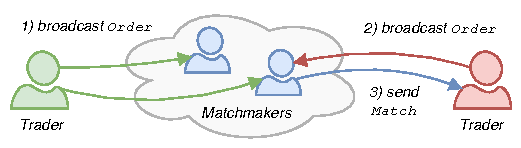
\includegraphics[width=0.7\linewidth]{xchange/assets/xchange_protocol_1}
	\caption{Phase I of the \ModelName{} trading protocol: traders (depicted in green and red) send new orders to matchmakers (shown in blue). Matchmakers notify traders about matches for their orders. }
	\label{fig:matching_protocol_1}
\end{figure}

\subsection{Phase I: Order Creation and Matching} \label{sec:phase_matching}

During the first phase of the \ModelName{} protocol, traders create new orders (offers and requests) and send these orders to matchmakers.
Matchmakers match incoming orders with existing orders in the order book, and notify order creators about trading opportunities.
Figure~\ref{fig:matching_protocol_1} visualizes the operations performed by traders and matchmakers during this phase, and Listing \ref{alg:phase1} lists the pseudo-code associated with this phase.

When a trader intends to exchange assets that it holds with assets that it wants to have, it creates a new order by calling the \texttt{create\_order} procedure (line 1, Listing \ref{alg:phase1}).
Each order $ O $ created by trader $ t $ is uniquely identified by ($ PK_t, O_{ind} $) where $ PK_t $ is the public key of $ t $ and $ O_{ind} $ is an ordinal positive integer indicating the order's position in the sequence of all orders of $ t $.
Furthermore, $ O $ contains a timestamp, indicating when the order has been created, a timeout, which specifies how long the order should remain valid, and a boolean value indicating whether the order is an offer or a request.
Inclusion of the timeout prevents orders from being open for an indefinite amount of time.
The content of $ O $ is digitally signed by $ t $ with $ SK_t $, to ensure non-repudiation and authenticity.
Finally, $ O $ contains specifications on the assets that $ t $ desires to buy or sell.
This information is provided as a tuple of assets, or an \emph{asset pair}.
If Alice wants to sell 1 BTC for 1 ETH, she creates an offer with asset pair (1 BTC, 1 ETH).
Similarly, if Bob wants to buy 1 ETH for 1 BTC, he creates a request with asset pair (1 BTC, 1 ETH).
The order creator includes the new order in a \MsgOrder{} message and disseminates it to a subset of all matchmakers (line 6), according to an order dissemination policy (see Section~\ref{subsec:overlay_logic}).
%which then includes the order in their order book.
%\textbf{TODO: Is it required?} Modeling orders is also adopted by other systems in the domain~\cite{veit2003matchmaking}.

% 
%Once a trader has prepared $ O $, it embeds the data in an \TROrder{} transaction and submits it for inclusion in $ \mathcal{B} $. 
%The trader waits until the confirmation for the transaction's inclusion in the ledger. 
%Note that the time before a transaction is finalized on $ \mathcal{B} $ highly depends on the specifications of $ \mathcal{B} $, as it may range from a few milliseconds to hours. 
%If $ L $ uses a proof of work consensus mechanism like Bitcoin, this confirmation can take up to an hour \textbf{Note: Is it really 1 hour. In some sources it is said to be 10 mins.}. 

Traders are able to cancel an unfulfilled order $ O $ by sending a (signed) \MsgCancelOrder{} message with $ O_{ind} $ to matchmakers (line 6).
If a matchmaker receives such a message, it immediately deletes the cancelled order from its order book (line 13).

When a matchmaker $ m $ receives an \MsgOrder{} message (line 9), it extracts the order from the incoming message, validates its digital signature, and assesses correctness of the incoming order according to an order validation policy (see Section \ref{subsec:overlay_logic}).
If the incoming order is invalid or expired, $ m $ discards it and does not consider it for matching. 
If the incoming order is valid, it will be inserted in the order book of $ m $ and immediately matched with any existing orders with a mutual interest (line 16). 
If the matchmaker establishes a match, it informs the trader that created the incoming order about the trade potential.
In the situation that an order matches multiple orders, each matched order couple is considered as a different prospective trade. 
For instance, if an order of a trader $ t $ matches with $ n $ reciprocal orders, there are $ n $ potential trades in question, each of which includes $ t $ as one trading partner.
For each established match, the matchmaker sends a \MsgMatch{} message to the trader that creates the incoming order (line 18).
A \MsgMatch{} message contains full details on the matched orders.

%Upon the arrival of new orders, a matchmaker evaluates whether there are orders with overlapping interests. 
%Order matching can either be on a one-to-one basis (e.g., in a ride-hailing market, one driver is matched with one passenger) or one-to-$n$ (e.g., in a stock trading market a stock offer can be matched with multiple stock requests).

The receiver of a \MsgMatch{} message is called the \emph{initiator}.
The initiator fulfils an important role if the match leads to a trade.
%An initiator is needed to manage conflicts during the negotiation and executions of the trade, as to be discussed in the next phase of the protocol.
When trader $ t $ receives a \MsgMatch{} message from $ m $, it first checks whether its order is still valid, i.e., whether it still has an interest in trading the respective assets. 
If so, it remembers the matched order by adding it to a queue (line 22).
Otherwise, $ t $ sends a \MsgRejectMatch{} message back to $ m $ with a reason (line 24).
Upon reception of a \MsgRejectMatch{} by a matchmaker, it updates the status of the respective orders in their order book (line 34) and attempts to find new matches (line 35).

For each order, a trader $ t $ maintains a \emph{match priority queue} which contains the set of matched counterparties, nominated by matchmakers to $ t $. 
Each trader can have its own decision mechanism to select one trader amongst the others in the match priority queue.
An example decision mechanism would be to set a timer for the order and select the trader who has been nominated by the highest number of matchmakers when the timer expires. 
We motivate and elaborate on matching priority queues in Section \ref{subsec:match_priority_queue}.
We call the trader selected from the matching queue the \textit{counterparty} of a prospective trade.
Once $ t $ selects a counterparty, phase II of the \ModelName{} trading protocol starts and the initiator verifies the counterparty (line 31). 
Furthermore, the initiator reserves (\enquote{locks}) these assets to the counterparty which prevents the situation where it would incorrectly respond to a \MsgTrdProp{} message for a specific order while having an outstanding trade proposal for the same order.
%This prevents an order from being fulfilled twice.

\begin{figure}[h]
	\centering
	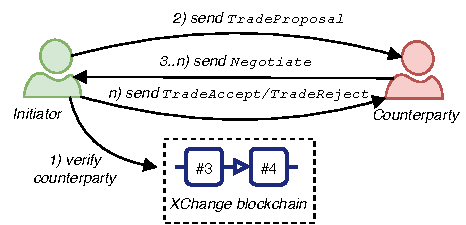
\includegraphics[width=0.6\linewidth]{xchange/assets/xchange_protocol_2}
	\caption{Phase II of the \ModelName{} protocol: two matched traders negotiate a trade.}
	\label{fig:matching_protocol_2}
\end{figure}

\subsection{Phase II: Trade Negotiation}
\label{sec:phase_negotiation}

The second phase of the \ModelName{} trading protocol is illustrated in Figure \ref{fig:matching_protocol_2} and formalized in Listing \ref{alg:phase2}.
During this phase, traders carry out off-chain trade negotiation with a sequence of network messages, without the involvement of matchmakers or other parties.
%The \MsgTrdProp{} message includes both the initiator's and counterpart's original orders.
%Even so, note that the initiator may change the amount of the assets to be exchanged, e.g., if a part of its order is already fulfilled. 
When an initiator has selected a counterparty for a potential trade, it first validates the counterparty by checking whether it holds responsibility during one of its ongoing trades (line 2, Listing~\ref{alg:phase2}).
Recall that a counterparty holds responsibility if it is their turn to initiate a payment to another party during an ongoing trade.
This can be verified by inspection of the transactions on $ \mathcal{B} $ that involves the counterparty.
Note that the presence of a \TRPayment{} transaction on $ \mathcal{B} $ is not enough to ensure that a party has actually transferred the promised assets.
Further inspection of the transaction identifier inside the \TRPayment{} transaction is necessary, which involves a transaction lookup in another blockchain.
An initiator following the \ModelName{} trading protocol will not engage in a trade with a counterparty that holds some responsibility.
This is a crucial property to address counterparty fraud in \ModelName{}.

\begin{lstlisting}[firstnumber=1,caption={Phase II: Trade negotiation.},label={alg:phase2},captionpos=b,float=t,numbers=left,tabsize=2, basicstyle=\footnotesize\ttfamily, mathescape=true, emph={while, if, then, do, Procedure, record, send, receive, in, foreach, ignore, else},emphstyle=\bf, frame=TB]
Procedure verify_trader($ O, counterparty $):
if $ check\_responsibilities(counterparty, \mathcal{B}) $
send TradeProposal($ proposal $) to $ counterparty $
remove $ counterparty $ from $ match\_queues[O] $
else
$ select\_trader\_from\_queue(O) $

On receive of TradeProposal($ proposal $) or Negotiate($ proposal $) message by peer $ p $:
$ result $ $ \leftarrow $ $evaluate(msg.proposal) $
if $ result $ = ACCEPT:
send TradeAccept($ proposal $) to $ msg.sender $
if p is initiator:
start_trade()
if $ result $ = NEGOTIATE:
send Negotiate($ proposal $) to $ msg.sender $
if $ result $ = REJECT:
send TradeReject($ proposal $) to $ msg.sender $
if p is initiator:
send RejectMatch($ proposal.O, proposal.O_m, reason $) to $ m \subseteq \mathcal{M} $
$ select\_trader\_from\_queue(O) $

On receive of TradeReject($ proposal $) message:
if initiator:
send RejectMatch($ proposal.O, proposal.O_m, reason $) to $ m \subseteq \mathcal{M} $
$ select\_trader\_from\_queue(O) $

On receive of TradeAccept($ proposal $) message by peer $ p $:
if p is initiator:
$ construct\_trade\_agreement(proposal)	$  # See phase III
\end{lstlisting}

If the initiator wishes to trade with a counterparty after the verification of their responsibilities, it sends a \MsgTrdProp{} message (line 3).
This message contains the order of the initiator, the identifier of the (matched) order of the counterparty, and a trade proposal.
When the counterparty receives a \MsgTrdProp{}, it has a chance to negotiate by sending \MsgTrdNegotiate{} message back to the initiator (line 15).
This might happen when the counterparty already fulfilled a part of their order and the initiator proposes to trade more assets than the counterparty is willing to.
This situation could occur if the matchmaker has outdated information on the status of the counterparty's order.

Trade negotiation may continue by an exchange of \MsgTrdNegotiate{} messages between the initiator and the counterparty, until one of the two sides eventually accept or reject the last negotiation offer by a \MsgTrdAccept{} or \MsgTrdReject{} message, respectively.
If one of the parties has sent a \MsgTrdAccept{} message, the initiator immediately starts the preparation of trade, entering phase III of the trading protocol (line 29). 
%If the counterparty accepts a trade proposal, it only sends a \MsgTrdAccept{} and waits for the initiator to start the construction of a trade agreement (during the next phase of the protocol).
In the situation where one side has sent \MsgTrdReject{} message, the initiator will send a \MsgRejectMatch{} message to the matchmaker to inform them about the failed negotiation, and select a new counterparty from the match priority queue, if available (lines 19 and 25).
The outcome of the negotiation phase is an asset pair which specifies which and how many assets will be exchange between the involved traders.

%\textbf{TODO: Rethink this part!, Do we really need to inform matchmakers? Can we just select another peer from the matching queue?}

%\textbf{TODO: I removed the check for fulfillment of order from the description, because I think it is not needed. \textit{c.u.i.}}

%
%
%
%Assume that trader $ A $ receives a \texttt{match} message from a matchmaker, matching one of their requests with an offer created by another trader $ B $.
%First, $ A $ checks the current state of their matched buy order since it could have been fulfilled already or expired.
%For instance, this happens when an order has been completed but matchmakers that have this order included in their order book are not notified about this fulfillment, leaving the fulfilled order in their order book and eligible for matching (see step X).
%If request of $ A $ is open and has not expired yet, it checks whether $ B $ is already involved in a trade with another trader.
%This should be detected with a linear scan of the distributed ledger $ \mathcal{L} $ and an inspection of all blocks created by $ B $.
%XChange stores full trade details in such a way that is it possible to detect whether a specific trader is currently involved in a trade.
%The exact specifications of this checks are outlined in Section X.\todo{Where?}
%If $ B $ is already trading with another party, $ A $ declines the \texttt{match} message and informs the matchmaker about this.
%The property to only be involved in a trade with a single counterparty at once is cardinal to limit the effectiveness of fraud, which we discuss in Section \ref{sec:security}.
%There could also be other reasons why $ A $ does not want to trade with $ B $.\todo{clearing policy}
%For example, $ A $ might prefer to only trade assets with traders that are geographically nearby.
%
%If $ A $ is willing to trade with trader $ B $,  $ A $ sends a \texttt{TradeProposal} message to $ B $.
%This message contains the intended asset quantity that $ A $ wants to exchange with $ B $.
%For instance, if $ A $ wants to buy 1 BTC for \$100 and $ B $ sells 2 BTC for \$200, $ A $ will send a trade proposal to buy 1 BTC for \$100.
%When $ B $ receives the \texttt{TradeProposal} message, it verified that its matched order is not fulfilled already or expired.
%$ B $ also determines whether $ A $ is currently involved in a trade, and whether there are any other reasons not to trade with $ A $.
%A trade proposal is now either accepted by sending a \texttt{AcceptProposal} message to $ B $, or rejected by sending a \texttt{RejectProposal}.
%When $ A $ receives an \texttt{AcceptProposal} message from $ B $, both traders will prepare for asset exchange and enter phase III.
%If $ A $ receives a \texttt{RejectProposal}, it informs the matchmaker about this event which then updates their order book accordingly.
%Alternatively, $ B $ can send a \texttt{CounterProposal} message back to $ A $, which contains a different proposal for the quantities to trade (if an order is already fulfilled partially).
%This counter proposal can then either be accepted or rejected by $ A $, by sending an \texttt{AcceptProposal} or \texttt{RejectProposal} message respectively.

\begin{lstlisting}[firstnumber=1,caption={Phase III: Constructing a trade agreement between an initiator and a counterparty.},label={alg:phase3},captionpos=b,float=t,numbers=left,tabsize=2, basicstyle=\footnotesize\ttfamily, mathescape=true, emph={while, if, then, do, Procedure, record, send, receive, in, foreach, ignore, else},emphstyle=\bf, frame=TB]
Procedure construct_trade_agreement($ proposal $)
$ A_{partial} \leftarrow proposal.to\_agreement() $
$ A_{partial}.add\_wallet\_info() $
send PartialAgreement($ A_{partial} $) to $ proposal.counterparty $

On receive of PartialAgreement($ A_{partial} $) message:
$ A \leftarrow A. add\_wallet\_info() $
send Agreement to $ A_{partial}.initiator $

On receive of Agreement($ A $) message:
$ \mathcal{B}.publish(A) $
$ trade \leftarrow A.to\_trade() $
insert $ trade $ in $ trades $
$ send\_payment(trade) $ # See phase IV
\end{lstlisting}

\begin{figure}[h]
	\centering
	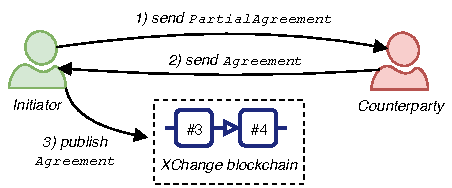
\includegraphics[width=0.6\linewidth]{xchange/assets/xchange_protocol_3}
	\caption{Phase III of the \ModelName{} protocol: the initiator and counterparty construct a trade agreement, which is published on the \ModelName{} blockchain by the initiator.}
	\label{fig:matching_protocol_3}
\end{figure}

\subsection{Phase III: Constructing a Trade Agreement} \label{sec:phase_agreement}

In the third phase of the trading protocol, traders enter into an irrevocable trade agreement and publish this agreement on the \ModelName{} blockchain.
This phase is visualized in Figure \ref{fig:matching_protocol_3} and formalized in Listing \ref{alg:phase3}.

When one of the parties accept the trade proposal, the initiator starts the third phase of the trading protocol by constructing a partial trade agreement, including local information regarding the upcoming trade (line 1, Listing~\ref{alg:phase3}).
This information includes the wallet address(es) of the initiator where the counterparty is expected to send assets to, the public keys (identifiers) of both traders, and the asset pair that is negotiated during the negotiation phase.
The trade agreement also contains information on whether incremental settlement is used, and if so, the number of expected payments originating from each side.
The initiator embeds this information in a \MsgPartialAgreement{} message, signs it, and sends to the counterparty (line 4).
When the counterparty receives the \MsgPartialAgreement{} message, it verifies the included information and creates an \MsgAgreement{} message which includes the wallet address(es) of the counterparty (line 6-8).
The counterparty signs the \MsgAgreement{} message and sends it back to the initiator, who then publishes the dual-signed trade agreement on $ \mathcal{B} $ (line 11).
Each trade agreement contains a \emph{publication deadline}.
If the trade agreement is published on $ \mathcal{B} $ after the publication deadline passed, the trade agreement is considered invalid.
Inclusion of this deadline addresses the attack scenario where an initiator purposefully withholds a dual-signed trade agreement to avoid taking responsibility in the trade specified by the agreement.
%The trade initiator is responsible for sending the first \MsgWallet{} message. 

%Once the parties have exchanged their wallet information, they both create a \TRAgreement{} transaction on $ \mathcal{L} $.
%This transaction includes the public identifiers, wallet information of both traders, and a trade agreement that includes the number of assets each party committed to pay.
%If the distributed ledger $ \mathcal{L} $ supports bilateral transactions where both parties could sign a single transaction, the parties only have to create one \TRAgreement{} transaction. 
%Even though the \textit{counterpart} can sign the transaction first, it is the \textit{initiator}'s responsibility to create the first \TRAgreement{} transaction. 

\begin{lstlisting}[firstnumber=1,caption={Phases IV: Execution of a trade.},label={alg:phase4},captionpos=b,numbers=left,float=t, tabsize=2, basicstyle=\footnotesize\ttfamily, mathescape=true, emph={while, if, then, do, Procedure, record, send, initiate, receive, in, foreach, ignore, else},emphstyle=\bf, frame=TB]
Procedure send_payment(trade)
$ payment \leftarrow trade.get\_next\_payment() $
$ payment.txid \leftarrow conduct\_payment(payment) $ # Transfer assets on blockchain
$ \mathcal{B}.publish(payment) $
send Payment($ payment $) to $ trade.counterparty $
if $ trade.complete() $:
$ construct\_trade\_done(trade) $ # See phase V

On receive of Payment($ payment $) message by peer $ p $:
$ trade \leftarrow payment.trade\_id $
$ valid \leftarrow payment.validate() $ # Is the payment initiated by the other side?
if $ valid $ and not $ trade.complete() $:
$ send\_payment(trade) $
elif $ valid $ and $ trade.complete() $ and is initiator:
$ construct\_trade\_done(trade) $ # See phase V
\end{lstlisting}

\begin{figure}[h]
	\centering
	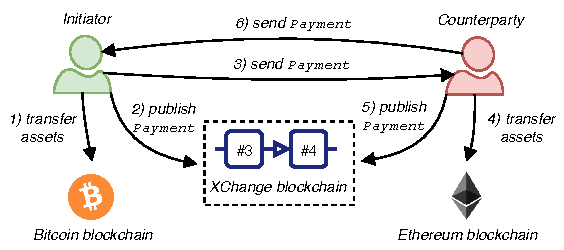
\includegraphics[width=0.7\linewidth]{xchange/assets/xchange_protocol_4}
	\caption{Phase IV of the \ModelName{} protocol: The trade is executed by a sequence of payments. In this figure, Bitcoin are exchanged with Ethereum assets, and the trade consists of two payments.}
	\label{fig:matching_protocol_4}
\end{figure}

\subsection{Phase IV: Trade Execution} \label{sec:phase_execution}

During the fourth phase of the \ModelName{} trading protocol, parties execute the trade and exchange assets in accordance with the trade agreement.
This phase is visualized in Figure~\ref{fig:matching_protocol_4} and the pseudo-code is provided in Listing \ref{alg:phase4}.

A trade usually consists of two payments (asset transfers), but more payments are required if the parties agreed on using incremental settlement.
%In this section, we consider a generalized trade where both parties make payment to each other.
The initiator always has the responsibility to make the first payment in a trade.
%Having signed the \TRAgreement{} transaction, the initiator of the trade cannot create any other record in the ledger until it makes the payment.
The initiator initiates a payment $ p $ by initiating an asset transfer on the blockchain that hosts the assets subject to trade (line 3, Listing~\ref{alg:phase4}).
This should result in a transaction identifier associated with the payment, say $ tx_p $.
The initiator then publishes the payment information on $ \mathcal{B} $ which includes $ tx_p $.
The \TRPayment{} transaction contains sufficient information for the counterparty to assess whether the initiator actually made the payment.
The transaction also includes a reference to the trade agreement.
The initiator then sends a \MsgPayment{} message to the counterparty to inform them about the payment (line 5).
The counterparty now polls its asset wallet to verify whether the promised assets have arrived (line 11).
If so, the counterparty initiates a payment back to the initiator.
This process repeats until all payments have been made and all assets have been transferred between the initiator and the counterparty.
At that point, the initiator finalizes the trade during the last phase of the trading protocol (lines 7 and 15).

%The counterpart may choose to wait for the initiator to make the payment first. 
%However, if the initiator makes the payment, creates the relevant record in the ledger and send the \MsgPayment{} message; the counterpart cannot create any other record in the ledger until it makes the payment.

%During the execution of a trade, the trader who makes the first payment takes a risk since the counterpart may leave the network after receiving the first payment.
%\ModelName{} has obstructive features to discourage such behavior. 
%First of all, when a party is next to make a payment, it is easily detected by a linear search in $ \mathcal{L} $. 
%For a party to continue using \ModelName{} and engage in other trades, it has to finalize the ongoing trade first. 
%Secondly, to reduce the value at risk, \ModelName{} supports \emph{incremental settlement}, where a single asset transfer is split up into several payments.
%The value of $ n $ should be increased when more value is exchanged, and initial risk-taking is higher.
%Incremental settlement decreases the value at risk but may prolong the overall trade.

\begin{figure}[h]
	\centering
	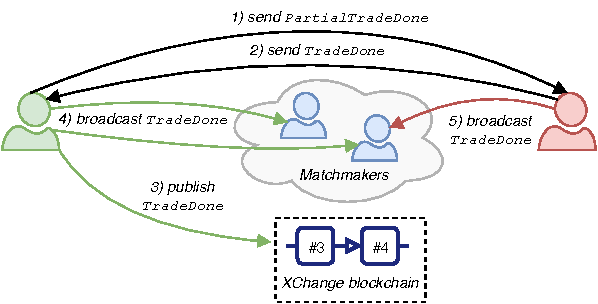
\includegraphics[width=0.7\linewidth]{xchange/assets/xchange_protocol_5}
	\caption{Phase V of the \ModelName{} protocol: The trade is finalized and matchmakers are informed about the conducted trade.}
	\label{fig:matching_protocol_5}
\end{figure}

\subsection{Phase V: Trade Finalization}
\label{sec:phase_finalization}
Once both parties have completed all payments and have created the \TRPayment{} transaction on $ \mathcal{B} $, they finalize the trade using a dual-signed transaction.
\ModelName{} explicitly finalizes, or \enquote{closes} a trade between two parties in order for others to quickly verify that a trade has been completed successfully, without having to verify individual \TRPayment{} transactions.
This process is visualized in Figure~\ref{fig:matching_protocol_5} and the associated pseudo-code is given in Listing~\ref{alg:phase5}. % is similar to the construction of a trade agreement (see Section~\ref{sec:phase_agreement}).
The initiator of a trade first sends a signed \MsgPartialTradeDone{} message to the counterparty (line 3, Listing~\ref{alg:phase5}).
This message is sent to the counterparty and contains the identifiers of the \TRAgreement{} and all \TRPayment{} transactions included on $ \mathcal{B} $.
Upon reception of this message by the counterparty, it signs the partial \MsgPartialTradeDone{} (line 6) and informs the matchmakers about the completed trade (line 8).
The counterparty then sends a \MsgTradeDone{} message back to the initiator (line 7).
When the initiator receives this message, it publishes the dual-signed trade finalization in a \TRTradeDone{} message on $ \mathcal{B} $ (line 11) and informs matchmakers about the completed trade (line 12).
%Finally, both parties involved in a completed trade broadcast the \TRTradeDone{} message to the matchmakers.
When a matchmaker receives a \MsgTradeDone{} message, it updates the status of the orders of the initiator and counterparty in their order book.

\begin{lstlisting}[firstnumber=1,caption={Phases V: Finalization of a trade.},label={alg:phase5},captionpos=b,numbers=left,float=t, tabsize=2, basicstyle=\footnotesize\ttfamily, mathescape=true, emph={while, if, then, do, Procedure, record, send, initiate, receive, in, foreach, ignore, else},emphstyle=\bf, frame=TB]
Procedure construct_trade_done(trade)
$ D_{partial} \leftarrow trade.to\_trade\_done() $
send PartialTradeDone($ D_{partial} $) to $ trade.counterparty $

On receive of PartialTradeDone($ D_{partial} $) message by peer $ p $:
$ D \leftarrow p.sign(D_{partial}) $
send TradeDone(D) to $ m \subseteq \mathcal{M} $
send TradeDone(D) to $ trade.initiator $

On receive of TradeDone($ D $) message:
$ \mathcal{B}.publish(D) $
send TradeDone(D) to $ m \subseteq \mathcal{M} $

On receive of TradeDone($ D $) message by matchmaker $ m $:
$ update\_order\_book(D) $
\end{lstlisting}

\subsection{Security Analysis} \label{sec:analysis}
We now present a basic security analysis of the \ModelName{} trading protocol and analyse the consequences of an adversarial trader that diverts from the protocol.
%In Section~\ref{sec:blockchain_accounting}, we discuss desired specification of $ \mathcal{B} $.
We leave a discussion of the security guarantees of the blockchain used by \ModelName{} to other work since these guarantees highly depend on the specifications of $ \mathcal{B} $.
The following analysis highlights potential attacks during the \ModelName{} trading protocol where an adversarial party attempts to purposefully compromise assets or stale  the activity of ongoing trades.
%For each phase in the \ModelName{} trading protocol, we consider threats to security where a specific party can negatively impact another party.

\textbf{Order creation and matching (phase I)}.
During the first phase, matchmakers may intentionally match orders according to their own desires.
For example, a matchmaker could give preferential treatment to orders made by specific traders, and report better matches for their orders.
However, since a trader disseminates new orders to multiple matchmakers simultaneously, there is a high probability that at least one matchmaker honestly reports matches back to the trader.
This probability increases if the order is sent to more matchmakers after its creation.

\textbf{Trade negotiation (phase II)}.
During the second phase, a trader first verifies the responsibilities of a counterparty before sending out a \MsgTrdProp{} message.
This is a key mechanism to limit counterparty fraud.
If $ t $ skips this verification, it opens a window of opportunity for the counterparty to commit fraud with multiple parties simultaneously, including $ t $.
If $ t $ acts rational, it is in their best interest to perform this verification by inspecting the outstanding trades of the counterparty to lower the risk of losing assets.

During the trade negotiation, any party can leave ongoing negotiations without repercussions by sending a \MsgTrdReject{} message to the other side.
This includes the situation where one of the parties does not respond with a \MsgTrdNegotiate{} or \MsgTrdAccept{} message in a timely manner.
The party that left the negotiations can now start new negotiations with another potential trading partner.
%Sending a \MsgTrdAccept{} will cause the initiator to start the construction of a trade agreement.

\textbf{Constructing a trade agreement (phase III)}.
While constructing a trade agreement, the initiator does have an incentive to defer the publication of a dual-signed trade agreement on $ \mathcal{B} $.
Specifically, as soon as the trade agreement is published on $ \mathcal{B} $, the initiator takes on responsibility during the agreed trade.
Inspection of the responsibilities of the initiator by others will reveal his position in the agreed trade, and other parties will refuse to trade with the initiator.
To ensure that the initiator publishes the agreement in a timely manner on $ \mathcal{B} $, the trade agreement contains a publication deadline (see Section~\ref{sec:phase_agreement}).
A trade agreement published after its publication deadline by the initiator is considered invalid by others, and the two parties that signed the expired agreement will not continue to the next phase of the trading protocol.
The publication deadline also forces the counterparty to respond to an incoming \MsgPartialAgreement{} message in a timely manner.

\textbf{Trade execution (phase IV)}.
During trade execution, a trader $ t $ might refrain from initiating a payment to the counterparty after having received assets from the counterparty.
However, other rational traders will not engage in a trade with $ t $ until $ t $ has passed on its responsibility.
Since \ModelName{} assumes that the identity of each trader is verified, $ t $ cannot easily re-enter the network under a new identity when it has committed fraud.
Also note that rational traders are not likely to refrain from publishing their \TRPayment{} transaction on $ \mathcal{B} $, since doing so will pass on their responsibility during an ongoing trade.

\textbf{Trade finalization (phase V)}.
When a trade between two parties enters the finalization phase (see Section~\ref{sec:phase_finalization}), all required payments have been made and all required \TRPayment{} transactions have been published on $ \mathcal{B} $.
Even if one of the parties actively delays the finalization phase, others can still assess that the trade has been completed by inspection of the last \TRPayment{} transaction.

%On one hand, an initiator might refuse to initiate the construction of a trade agreement, by not sending a \MsgPartialAgreement{} to the counterparty.
%This does not negatively impact the counterparty since there is no public, irrefutable evidence of the negotiation outcome and the prospective trade at this point. % not incur any responsibility
%On the other hand, the counterparty could refuse to sign for the (partial) trade agreement, or the initiator could withhold the dual-signed trade agreement.
%In this case, the initiator could \enquote{unlock} the assets they reserved for the counterparty, exchange these assets with another (honest) trader, and decide not to publish the trade agreement on $ \mathcal{B} $ once the counterparty sends the dual-signed trade agreement back.
%Finally, we consider the scenario where 

%\textbf{Counterparty fraud analysis}.
%Full accounting of trade information within transactions on $ \mathcal{L} $ is the cardinal property to limit the effectiveness of counterparty fraud.
%Recall that counterparty fraud happens when a party fails to meet their obligations to another party during a trade, e.g., when a trader purposefully does not initiate a payment.
%We now provide an informal proof that a trader cannot conduct this form of fraud with multiple parties at once.

%\ModelName{} supports concurrent trades.
%However it establishes strict trade rules for parties to limit the effectiveness of counterparty fraud. 
%We make the following analogy to prove the concurrency of trades. 
%We conceptualize each specific trade as a process of \textit{token-passing} between two peers. 
%Holding a token at a specific time means having a \textit{responsibility} to perform a task. 
%The token appears at the hands of the initiator of a trade when the traders sign a \TRAgreement{} transaction on $ \mathcal{L} $, and disappears when both parties create \TRTradeDone{} transactions. 
%When a peer performs its task, it passes the token to the counterpart of the trade, by a simple linear scan of $ \mathcal{L} $. 
%Any peer in the network can validate at any time if a specific trader holds a token.
%In other words, when it is the turn of a trader to make a move within the context of a trade (such as initiation, payment or finalization), it cannot hide this responsibility from the others.
%Holding a token prevents other peers from passing their tokens.
%Nonetheless, a trader can still start a trade \textit{at its own risk} with a party already engaged in an ongoing trade.

%\begin{figure}[t]
%	\centering
%	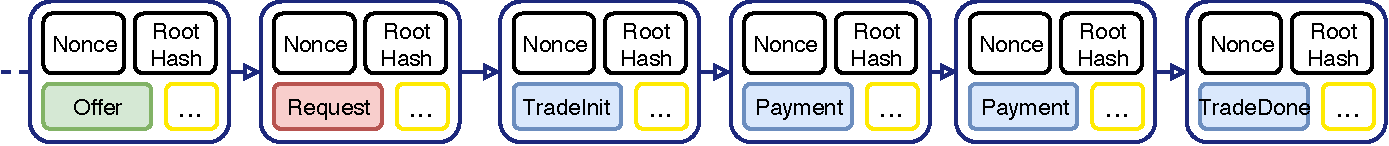
\includegraphics[width=\linewidth]{assets/trade_normal_ledger}
%	\caption{TODO.}
%	\label{fig:trade_normal_ledger}
%\end{figure}

%\begin{itemize}
%\item \textbf{Proof of assets}. A trader can only enter into agreement if it has enough assets to satisfy the terms of the agreement.

%\ModelName{} guarantees that a trader cannot make an agreement that he is unable to adhere to. There are a couple of ways to ensure it. 
%First of all, when a trader informs the matchmakers about an order, the matchmakers could validate the order by checking whether the trader has what it promises to have.
%Secondly, after the trade negotiations, when the parties of the trade try to enter into an agreement, they exchange their wallet information by \MsgWallet{} messages. 
%Any party of the trade can validate the existence of promised assets in the wallet of the counterpart.
%Thirdly, during the execution of the trade, just before a trader makes a payment, it can check the account of the counterpart. 
%Fourthly, the party, who executed the payment and created the related ledger record (\TRPayment{}) before the counterpart, enables the other traders in the network to see that the counterpart is obliged to make the payment. 
%To see this, assume there are two ongoing trades in the network, one between traders $ A $ and $ B $, and the other between traders $ B $ and $ C $. 
%Assume also that $ A $ has rendered its payment before $ B $ and created the relevant transaction in $ \mathcal{L} $. 
%Now consider the trade between $ B $ and $ C $. 
%Even if $ B $ can prove the existence of its assets for the transaction between $ B $ and $ C $, its assets might not be enough for fulfilling both of the trades. 
%However, in this case $ C $ would easily evaluate $ \mathcal{L} $ and, after seeing $ B $'s assets are enough, $ C $ refrains from agreement with $ B $.
% The state of holding a token can be evaluated by any peer in the network . 
% Holding a token prevents other peers to pass their tokens \textbf{TODO: Define rules}

%	\item (\textbf{Atomicity of a trade.}) An agreed trade is eventually cleared off, given that the traders continue making transactions. 
%	
%	\ModelName{} prevents a trader to start a new trade before fulfilling its responsibilities brought by currently ongoing trades. 
%	\ModelName{} also assumes that the traders are online and continue to make transactions. 
%	Therefore, a trader having at least one responsibility must fulfill one of its responsibilities when it makes a new transaction. 
%	Since the responsibilities of a trade is finite (agreement, payment and finalization) and it cannot start a new trade before finalizing the existing ones, an initiated trade is eventually cleared off.
%	\item (\textbf{Prevention of \todo{Find a better name} Denial of Service.}) If a trader fulfills its responsibilities, it cannot be locked by any other trader. 
%	
%	To prove this guarantee, we revisit the token-passing analogy. 
%	When a trader holds a token, the others prevent entering into trade with or carrying out their responsibilities to her. 
%	
%\end{itemize}

%\textbf{TODO: This subsection will provide proofs for the following:}
%\begin{itemize}
%\item a trader cannot make an agreement for something he does not have
%\item An agreed trade is subject to be finalized, or the party who does not fulfill its responsibilities 
%\end{itemize}

\section{The \ModelName{} System Architecture}
\label{sec:architecture}
We now present the \ModelName{} system architecture, visualized in Figure \ref{fig:mechanism_architecture}.
Each active peer in the \ModelName{} network runs a single implementation of this system architecture as a shared library.
We briefly explain each component and highlight how interaction proceeds between components.

\subsection{Network Layer}
\label{subsec:network_layer}
The network layer passes incoming messages to the overlay logic and routes outgoing messages to their intended destination.
This layer can be implemented using any networking library with support for peer-to-peer communication (for example, libp2p\footnote{https://libp2p.io}).
The \ModelName{} trading protocol does not make assumptions about the topology of the network layer, except for the fact that each peer should know the network address of some matchmakers that can match their orders.
In our implementation, we use a bootstrapping mechanism where new peers in the network immediately attempt to discover some available matchmakers.
The networking library manages this bootstrapping process.
%The order dissemination policy (see Section X) specifies how many matchmakers a trader should know.
Attacks targeted at the network layer (e.g., the Eclipse Attack~\cite{singh2006eclipse}) are beyond the scope of this work.
%We should note however that further optimizations can be made in network topology, depending on the domain to which MATCH is applied.
%This lowers generality and re-usability.
%The network has a random topology and each peer $ p $ maintains a connection to $ i $ other random peers.
The Sybil Attack is addressed by the requirement for strong identities, as discussed in Section \ref{sec:protocol}.

\begin{figure*}[t]
	\centering
	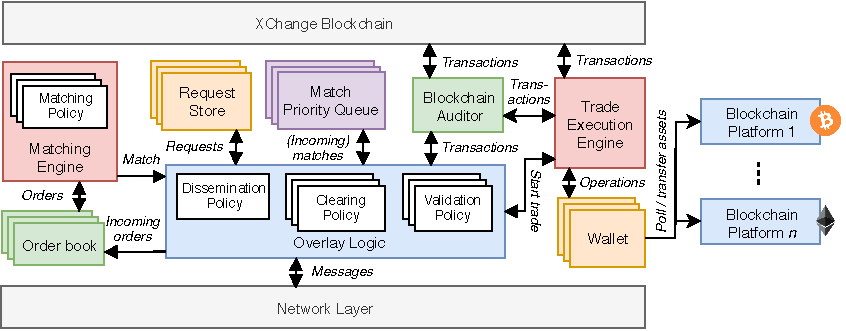
\includegraphics[width=\linewidth]{xchange/assets/xchange_architecture}
	\caption{The system architecture of \ModelName{}, our mechanism for generic trade at scale. Arrows between two components indicate interaction or data exchange.}
	\label{fig:mechanism_architecture}
\end{figure*}

\subsection{Overlay Logic}
\label{subsec:overlay_logic}
The \ModelName{} overlay logic (depicted in blue in~Figure \ref{fig:mechanism_architecture}) reacts to incoming network messages and optionally passes the information in these messages to the relevant components.
For example, an incoming order (embedded in an \MsgOrder{} message) is passed to the order book and stored there.
Similarly, the information in an incoming \MsgMatch{} message is passed to the match priority queue.
The overlay logic interacts with the trade execution engine when a new trade is about to start, e.g., when receiving a \MsgTrdAccept{} message.
It also passes information about an incoming \MsgPayment{} message to the trade execution engine.
The overlay logic defines three different policy types, for order dissemination, order validation, and (trade) clearing.
These policies are explained next.

\textbf{Dissemination policy}.
The dissemination policy specifies how a new order is disseminated to matchmakers.
It contains information to which matchmakers a new order should be send.
The number of matchmakers that receive a new order is also called the \emph{order fanout}.
Sending a new order to more matchmakers potentially speeds up the matching of this order, but it also increases the load on matchmakers since they have to process more incoming \MsgOrder{} messages.
%A performance analysis of decentralized order matching under different dissemination policies can be found in our other work.

\textbf{Clearing Policies}.
The clearing policies predicate whether a specific peer should send out a trade proposal to another trader, or accept an incoming trade proposal that it received (during phase II of the \ModelName{} trading protocol, see Section \ref{sec:phase_negotiation}).
\ModelName{} enables programmers to define distinct and multiple clearing policies for orders with differing specifications.
For example, a clearing policy could specify that a trader can only exchange assets with other traders that are within geographic proximity.
Another clearing policy could implement trading restrictions governed by regional or local legislation.
We have implemented the strategy that a trader only interacts with traders to do not hold any responsibility during trade as a clearing policy.
This policy is enabled by default.

\textbf{Validation Policies}.
The validation policies implement validation rules for new incoming orders.
Similar to the clearing policies, multiple validation policies can be applied to orders with differing specifications.
An order validation policy often takes into consideration the information in each order and determines whether this attribute data is valid with respect to a specific domain
%For example, a validation policy to verify stock trading orders should check whether the quantity of stocks that a trader wants to buy or sell is a positive number
(e.g.\ whether the quantity of stocks is non-negative).
The overlay logic immediately discards orders that are classified as invalid by any applied validation policy.

\subsection{\ModelName{} Blockchain}
%We discuss the details of the distributed ledger underlying \ModelName{} in the next section.
The \ModelName{} trading protocol assumes the availability of a blockchain on which full trade specifications are stored.
The popularity of the Bitcoin cryptocurrency bootstrapped the development of an extensive range of blockchain platforms with varying security and performance guarantees.
Most of these ledgers are designed to securely manage and transfer cryptocurrencies or digital tokens.
The distributed ledger used by \ModelName{} does not necessarily need the required security level of managing digital currencies.
Instead, we require a blockchain that merely allows for the tamper-proof storage of trade specifications.
We explore suitable blockchains for the \ModelName{} trading mechanism in Section \ref{sec:implementation}.

\subsection{Order Book}
\label{subsec:order_book}
An order book is a data structure that stores (active) orders.
It lists the specific assets that are being bought or sold within the market and provides traders with a convenient view of the current supply and demand.
Depending on the trading environment, orders in the order book often contains the identity of its creator, and sometimes the reputation scores of the order creator (for instance, eBay shows the trustworthiness of merchants).
%Figure \ref{fig:order_book} shows an example of an order book used in a stock trading market, with three bid orders and three ask orders.
%An order book often show orders in distinct lists, as visualized in Figure~\ref{fig:order_book}.
%This order book contains three buy orders and three sell orders.
When presenting an order book to traders, orders are usually sorted on one or more attributes, e.g., based on their price.
For orders with pricing information attached, the order book usually lists the \enquote{best} orders at the top.

In \ModelName{}, each matchmaker can operate multiple order books for different order types (coloured green in Figure~\ref{fig:mechanism_architecture}).
Specifically, orders exchanging the same asset pair are stored in the same order book.
An \emph{asset pair} specifies the pair of assets that are being traded in an order book and uniquely identifies each order book.
For example, an order book identified by the BTC/ETH asset pair contains orders that buy or sell Bitcoin and Ethereum gas.
%Since a buy order in the AAPL/USD order book is equivalent to a sell order in the USD/AAPL order book, \ModelName{} only maintains order books which asset pair is lexicographically sorted.
%Internally, it treats a buy order in the USD/APPL order book as a sell order in the APPL/USD order book.
%Likewise, a sell order in the USD/APPL order book is treated as a buy order in the APPL/USD order book.
Maintaining distinct order books at the same time enables order management with a single infrastructure across different trading domains.
%New order books can be created on demand when a matchmaker receives valid orders from the network.

%Market orders rarely end up in the order book as open order, since they are often fulfilled instantly.
%A defining metric used by traders is the difference between the price of the highest ask order and the price of the lowest bid order, also called the \emph{bid-ask spread}.
%For the order book shown in Figure \ref{fig:order_book}, the bid-ask spread is \$149.57 - \$149.54 = \$0.03.
%This metric also indicates market liquidity, the degree to which assets can be quickly bought or sold.
%A liquid market is often characterized by a low bid-ask spread.

%The number of different price levels at a specific time is called the \emph{order book depth}.
%Some markets ignore or reject orders with a price beyond a specific depth.\todo{example?}
%The order book depth is a metric used by traders to determine where the price of a particular asset could be heading in the near future.

%Centralized trading venues store their order book on one or more servers.
%The implementation of the order book and how the data is exactly stored, is determined by the market operator and rarely disclosed. %owned and maintained by the market operator.
%Some markets, like stock or (crypto)currency exchanges, have to deal with a high arrival rate of new orders.
%Efficient insertion of new orders in the order book and quick modification of existing ones is important to facilitate low-latency trading (usually within milliseconds).
%It is common to optimize order book operations so they can be carried out in $ O(1) $ or $ O(log\ n) $ time (where $ n $ corresponds to the number of ask or bid orders in the order book).

%As we will elaborate in Section \ref{sec:market_blockchain}, \ModelName{} explores market data stored on the distributed ledger (the blockchain) and aims to find orders created by other traders.
%When \ModelName{} discovers a new order, the validity of the order is checked.
%The validation function will verify if the order has not expired yet and whether it is valid with respect to the rules of the trading environment.
%Only if an order is deemed valid, it will be inserted in a local order book. % and if it is valid, it will be added to the local order book.
%Expired orders are automatically removed from a local order book.
%Newly inserted order book entries are passed to the order matching engine.
%When \ModelName{} discovers that the status of an order has changed, the corresponding order book entry is updated accordingly.

%This work does not focus on pricing mechanisms and decentralized price discovery.
%These topics are covered by related work in the field of economics\todo{cite}.
%We note however that such mechanisms often rely on specific order organizations or trading domain.
%Instead, our trading mechanism should be independent of the type of assets or services being traded.
%Various components of the architecture in Figure~\ref{fig:mechanism_architecture}, like the matching engine and the local order book, could be adapted to better match the trading environment in which \ModelName{} is being used.
%For the experiment presented in Section  we build a stock trading market with our architecture. % for real-world trading traces of the Apple stock symbol.
%The exact specification of pricing is likely to differ between different types of market (resource allocation within distributed computing, energy markets or ride-hailing).

\subsection{Matching Engine}
\label{subsec:local_order_book}
The matching engine (coloured red in Figure~\ref{fig:mechanism_architecture}) matches incoming new orders with existing orders in order books.
Marketplaces operated by a central authority often deploy an in-house order matching engine, fully controlled by the market operator.
DEXes sometimes integrate the order matching process in the transaction validation process.
In \ModelName{}, each matchmaker operates a matching engine and immediately attempts to match new incoming orders.
Established matches for an incoming order are passed to the overlay logic, embedded in a \MsgMatch{} message and sent to the order creator.

The matching engine can contain multiple \emph{matching policies}.
A matching policy predicates whether an offer and request match, and is applied to a single type of order book.
It takes a single offer and request as input and determines whether these orders match, based on their specifications.
In the context of cryptocurrency trading, whether two orders match depends on the asset price contained in the order.
%On the other hand, in a ride-hailing marketplace like Uber, matchmaking is usually based on the geographical distance between a driver and a passenger.
The most common matching strategy in financial markets is the \emph{price-time matching strategy}, where orders are first matched based on their price, and then based on order creation time in case of a tie-breaker (older orders are prioritized).
\ModelName{} allows programmers to define custom matching policies.
%The technicalities of this process are elaborated in Section~\ref{sec:implementation}.

\subsection{Request Stores}
To correctly process incoming \MsgTrdAccept{} and \MsgTrdReject{} messages during trade negotiation (phase II of the \ModelName{} trading protocol, see Section~\ref{sec:phase_negotiation}), \ModelName{} stores the state of outgoing \MsgTrdProp{} and \MsgTrdNegotiate{} messages.
The state of outgoing messages is stored in distinct \emph{request stores} (coloured yellow in Figure~\ref{fig:mechanism_architecture}).
For each outgoing message that has a state attached, a unique identifier is generated, a new request store containing this identifier is created and the generated identifier is appended to the outgoing message.
Traders that receive a message with this identifier are required to include the same identifier in their response message.
Incoming response messages with an unknown identifier are discarded and not processed further.
Each request store can have an optional timeout, indicating the duration after which the request store times out.
On timeout of a request store, it is deleted, and the overlay logic is notified about this event.

\subsection{Match Priority Queue (MPQ)} 
\label{subsec:match_priority_queue}
%Incoming \MsgMatch{} messages are stored in a matching priority queue and removed when this message is about to be processed.
%New match priority queues can be dynamically created when a peer receives a \texttt{match} message of a specific order for the first time.

After creating a new order, a trader can receive multiple \MsgMatch{} messages from matchmakers within a short period of time.
A basic approach is to process incoming \MsgMatch{} messages on a first-in-first-out (FIFO) basis.
However, this approach leaves the mechanism vulnerable to an attack where a malicious matchmaker is the first to send a specific \MsgMatch{} message with low quality to a trader, which is then immediately processed by this trader.
The trader might have received a better match from an honest matchmaker if it would have waited longer before processing incoming \MsgMatch{} messages.

This issue is addressed as follows: incoming \MsgMatch{} messages for a specific order are first collected and stored in MPQ, coloured purple in Figure \ref{fig:mechanism_architecture}.
When a trader receives the first \MsgMatch{} message for their specific order $ O_1 $, it creates a new match priority queue for $ O_1 $.
Each entry in the MPQ of order $ O_1 $ is a two-dimensional tuple $ (r, O_2) $ where $ r $ indicates the number of retries, and $ O_2 $ is the order that matches with $ O_1 $.
Removing items from the matching queue is first based on $ r $ (item with a lower value of $ r $ have a higher priority) and then based on the quality of the match (better matches have a higher priority).
The number of retries $ r $ in each entry $ (r, O_2) $ indicates how many times we tried to negotiate a trade with the creator of $ O_2 $.
This value is initially zero and incremented by one each time a trade proposal is denied for the reason that a counterparty does not have any unreserved assets.
Specifically, when a trader receives a \MsgTrdReject{} message for this reason from the creator of $ O_2 $ during trade negotiation for his own order $ O_1 $, it adds the entry $ (r + 1, O_2) $ to the MPQ of $ O_1 $.
%Since a trading partner might have quantity reserved in their order that is released later, we try to send another trade proposal later in this situation.

Before trade negotiation with a specific trader starts, incoming matches for each order are stored in MPQ for some duration $ W_m $, also called the \emph{match window}.
The value of $ W_m $ should be carefully considered: a high value of $ W_m $ increases the probability of receiving good matches but adds to the order completion time since a trader has to wait longer before sending out trade proposals.
On the other hand, decreasing the match window might lead to missing better matches.
When the match window expires, a trader removes an entry $ (r, O) $ from the MPQ, verifies the counterparty and sends out a \texttt{ProposeTrade} message to the trader that created $ O $ when the the trader wishes to trade with the counterparty (also see Section~\ref{sec:phase_negotiation}).
%To prevent traders from sending out \texttt{ProposeTrade} messages at roughly the same time (and thus increasing load on individual traders), we introduce a small \emph{propose window} $ W_p $ which is a random duration between the removal of an entry from a match queue, and sending out a \texttt{ProposeTrade} message.
Only when trade negotiation for an order fails or succeeds, the next entry is removed from the appropriate MPQ if there is still trading opportunity for order $ O $.
If $ O $ is fulfilled, the MPQ associated with $ O $ is deleted.

\subsection{Blockchain Auditor}
\label{subsec:ledger_auditor}
The blockchain auditor (coloured green in Figure~\ref{fig:mechanism_architecture}) inspects the transactions that are stored on the \ModelName{} blockchain and reports this information to the trade execution engine or the overlay logic.
Conceptually, it converts the information in transactions stored on the distributed ledger to domain-specific knowledge that can be used by different components.
For example, prior to trade negotiation between two traders, the overlay logic invokes the blockchain auditor to determine whether a trader $ t $ holds responsibility in an outstanding trade with another party (which is determined by inspecting the transactions which involve $ t $).

\subsection{Trade Execution Engine}
\label{subsec:trade_execution_engine}
The trade execution engine manages and controls the trading process.
It tracks the current state of a specific trade and interacts with the \ModelName{} blockchain to store trade agreement, payment specifications and trade finalizations.
%For example, upon reception of a \texttt{payment} message from a counterparty, it will poll wallets whether assets have been received and if so, initiates a payment to the counterparty if the trade has not been completed yet.

\subsection{Wallets}
\label{subsec:wallets}
\ModelName{} organizes different types of assets within wallets.
These wallets organize the information provided by external blockchain platforms (e.g., Bitcoin or Ethereum) in a generic manner.
Wallets are designed to store information on any digital asset such as cryptocurrencies or digital tokens.
Wallets expose functionality to transfer available assets to others, to query the current balance and to fetch past transactions.
Each wallet is uniquely identified by a \emph{wallet address}, usually a public key.
The addresses of wallets where assets should be sent to are included in a \TRAgreement{} transaction on the \ModelName{} blockchain.

\subsection{External Blockchain Platforms}
As outlined in the protocol description, the \ModelName{} blockchain stores full trade specifications.
\ModelName{} interacts with external blockchain platforms, such as the Bitcoin or Ethereum platform, to transfer assets to the counterparty.
Specifically, wallets invoke operations to query external blockchain platforms whether assets have been received, or to transfer assets.
%Settlement providers manage digital assets and carry out the operation of transferring these assets to others if instructed to do so.
%Notable examples are cryptocurrency networks such as Bitcoin or Ethereum, and financial institutions like banks.
%We assume that settlement providers are trusted parties and do not collude with an adversarial party.
%Many settlement providers provide a public interface to transfer assets to others or to query one's asset balance.
%By relying on the services of settlement providers, our trading mechanism supports generic trade of any digital asset, even beyond blockchain-based currencies and tokens.
%In \ModelName{}, asset exchange between two traders is a sequence of bilateral asset transfers that only involve both trading parties and settlement providers.
%This trading process is similar to how trade proceeds on many electronic marketplaces, like eBay.

\section{Blockchain-based Accounting of Trade Specifications}
\label{sec:blockchain_accounting}
The \ModelName{} trading protocol (see Section~\ref{sec:protocol}) requires a blockchain to store full trade specifications.
The popularity of blockchain technology has resulted in much interest to design and deploy distributed ledgers with different scalability and security guarantees.
In this section, we review different blockchain organizations and show which structures synergies with the \ModelName{} trading protocol.

%\begin{figure}[t]
%	\centering
%	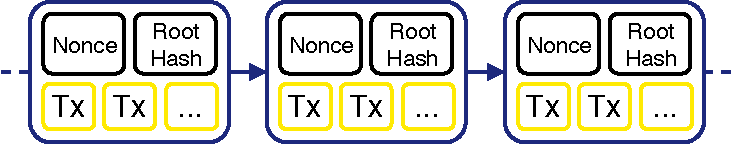
\includegraphics[width=.6\linewidth]{assets/bitcoin_ledger}
%	\caption{A blockchain ledger with a linear organization of blocks, used by Bitcoin and Ethereum. Each block contains a one or more of transactions, a nonce (used by the consensus mechanism) and the root hash of the Merkle tree with all hashes of transactions within the block.}
%	\label{fig:bitcoin_ledger}
%\end{figure}

\subsection{Traditional Blockchain Ledgers}
%Widely used blockchain applications like Bitcoin and Ethereum deploy a single and linear ledger, fully maintained by individuals in the network itself.
%Figure \ref{fig:bitcoin_ledger} shows a simplified representation of such a blockchain, with three blocks.
%Each block contains one or more transactions, a nonce (which is used by the consensus mechanism to secure the ledger) and the root hash of the Merkle tree with all hashes of transactions in the block.
%By inclusion of this root hash, one can verify in $ O(log\ n) $ time whether a transaction is included in a specific block.
%Each block has a specific height, indicating the index of the block with respect to the first block in the ledger (which has a height of 1).

% is crucial to build trust in a network with mutual distrust amongst members. %but severely limits throughput of the overall system and increases complexity.
In most traditional blockchain ledgers, there is a global consensus mechanism that periodically determines a leader amongst all consensus participants, or \emph{miners}.
This leader is then allowed to extend the blockchain with exactly one block.
In the Bitcoin network, a new block is appended roughly every ten minutes~\cite{nakamoto2008bitcoin}.
%Users participating in the consensus mechanism are called \emph{miners}.
For Bitcoin and Ethereum, each miner in the network attempts to solve a computational puzzle and the first miner to solve the puzzle can append a new block to the blockchain ledger (Proof-of-Work).
Verifying the correctness of a proposed solution is computationally efficient and can be performed in $ O(1) $ time.
The difficulty of the computational puzzle grows with the overall computing power of the network.
%As the overall computing power of the network grows, so does the difficulty of the puzzle.
%The miner that is selected by the consensus mechanism, influenced by the amount of computing power each individual invested in the network (also called Proof-of-Work consensus).
%Selecting a miner based on computing power is also called Proof-of-Work.
Other consensus mechanisms might select a leader based on the miner's stake in the network (Proof-of-Stake) or by election of a committee that produces blocks (Delegated Proof-of-Stake)~\cite{bentov2014proof}.
%Without a \emph{global} (network-wide) consensus mechanism that controls the growth of the blockchain ledger, the network would be void of agreement on the current blockchain state.
For \ModelName{}, and even within Internet-of-Things applications in general, we consider the usage of blockchain ledgers secured by global consensus impractical for the following two reasons.\footnote{Still, the \ModelName{} trading protocol can leverage any distributed ledger that is secured by global consensus and has accounting capabilities.}

\begin{enumerate}
	\item \textbf{Inefficient.} Reaching a global, network-wide consensus is often an expensive process in terms of CPU power, bandwidth usage and storage requirements.
	It negatively impacts the throughput of a blockchain in terms of finalized transactions per second.
	%This makes it impractical for resource-constrained devices operating within the Internet-of-Things to maintain a blockchain ledger secured by global consensus\todo{cite}.
	The theoretical throughput of a blockchain ledger is often bounded by a constant value.
	Gervais et al. found that global consensus mechanisms based on computing power (Proof-of-Work) can achieve up to around 60 transactions per second before security issues arise~\cite{gervais2016security}.
	Considering the throughput needed to process payments at a global scale, many blockchains are by far not scalable enough to provide viable alternatives for financial use-cases such as asset marketplaces.
	\item \textbf{Transaction fees.} To incentive participation in the consensus mechanism, miners are rewarded by transaction fees.
	These transaction fees are covered by users that initiate a transaction.
	Depending on the blockchain used by \ModelName{}, the transaction fees required to get the transactions included during a trade might be relatively high, especially if a trader only desires to exchange a few assets with relatively low value.
	%Furthermore, a trader has to pay transaction fees to include a new order in the \ModelName{} blockchain and when cancelling existing orders.
	Transaction fees potentially make asset trading with \ModelName{} a costly process.
\end{enumerate}

%The second issue is that it can take a considerable amount of time before new buy and sell orders are included within a block on the ledger.
%Even though the interval between block creation can be as low as a few seconds, it is still unsuitable for situations that require near-instant confirmation of market activity~\cite{schuh2015bitshares}.
%Examples of such situations include real-time bidding and high-frequency trading.

%The third issue is that traders often have to pay a fixed or percentage-based fee to get their orders included on the ledger.
%This fee is then collected by the users who donate their computing power to keep the ledger secure.
%While centralized marketplaces often charge transaction fees too, trading in large volume is costly on most blockchain-based marketplaces.

%Second, it is questionable whether reaching a global consensus on all market activity is an appropriate mechanism to effectively facilitate real-world trading.
%In particular, asset exchange often proceeds on segmented markets.
%For example, stock trading venues operate highly isolated from each other, based on geographical location.
%Another example is local energy trading where interactions are limited to a neighbourhood or a geographical district (since it is inefficient to transmit bought energy over a large distance)~\cite{mengelkamp2017trading}.
%We believe that establishing a global consensus on aggregated information, generated by traders on isolated markets, is unnecessary.

\subsection{DAG-based Blockchains}
As an attempt to increase the throughput of distributed ledgers, various platforms reorganize the structure of their blockchain and maintain a Directed Acyclic Graph (DAG) structure instead~\cite{sompolinsky2018phantom}.
Notable applications that deploy a DAG structure include IOTA, Nano and Dagcoin~\cite{popov2016tangle}~\cite{lerner2015dagcoin}.
Its distinguishing property is that each transaction can be referenced by multiple other ones and as such, it forms a DAG of transactions.
Transactions in a DAG are linked, and each transaction verifies one or more prior transactions.

Since DAG-based ledgers allow for more efficient and localized consensus models, we argue that they are better suited for the accounting of trade specifications in \ModelName{}.
However, many DAG-based ledgers violate on decentralization.
Since some implementations are not properly tested at scale yet, appending transactions to the ledger is controlled by a centralized coordinator (e.g., IOTA).
Other implementations compromise on decentralization by assembling a fixed group of witness nodes that verify transactions and include them in the ledger (e.g., Nano and Dagcoin).
We specifically aim to avoid authorities with leveraged permissions to prevent (strategic) censorship of the transactions that are submitted to the \ModelName{} blockchain.

\subsection{TrustChain: A Scalable Blockchain for Accounting} \label{sec:trustchain}
Based on the idea of DAG-based blockchains, Otte et al. designed and deployed TrustChain, a blockchain that is optimized for lightweight, tamper-proof accounting of data elements~\cite{otte2017trustchain}.
The key idea is that individuals maintain and grow their \emph{individual ledger} with transactions they have initiated and have been involved in.
Individual ledgers are intertwined (i.e.\ entangled) with each other and form a DAG structure.
TrustChain does not aim to prevent fraud like the double spend attack but instead guarantees eventual \emph{detection} of such fraud.
This yields superior scalability compared to other ledgers but allows for the situation where some fraud targeted at the blockchain layer might go undetected for some time.
Individuals in TrustChain are not required to store all transactions in the network and might choose to store different parts of the global DAG ledger.
Consensus is only reached between interacting parties and not on a global scale.

\begin{figure*}[t]
	\centering
	\begin{subfigure}[t]{.33\textwidth}
		\centering
		\captionsetup{width=.9\linewidth}
		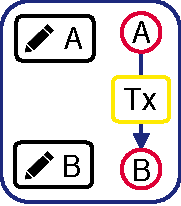
\includegraphics[width=.35\linewidth]{xchange/assets/trustchain_tutorial_1}
		\caption{A block with a transaction (\emph{Tx}) between two users ($ A $ and $ B $). Each block contains a single transaction, two digital signatures and two digital identities.}
		\label{fig:trustchain_tutorial_1}
	\end{subfigure}%
	\begin{subfigure}[t]{.33\textwidth}
		\centering
		\captionsetup{width=.9\linewidth}
		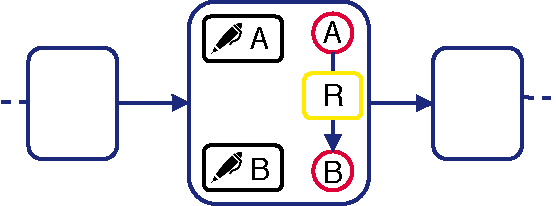
\includegraphics[width=\linewidth]{xchange/assets/trustchain_tutorial_2}
		\caption{A blockchain of transactions. Each block in the chain contains a hash that describes the prior block.}
		\label{fig:trustchain_tutorial_2}
	\end{subfigure}%
	\begin{subfigure}[t]{.33\textwidth}
		\centering
		\captionsetup{width=.9\linewidth}
		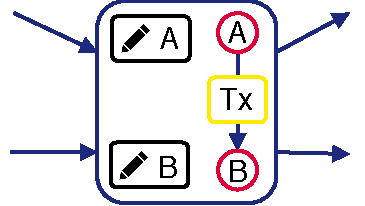
\includegraphics[width=.7\linewidth]{xchange/assets/trustchain_tutorial_3}
		\caption{To increase security, each block also references the previous block in the chain of the other transaction participant.}
		\label{fig:trustchain_tutorial_3}
	\end{subfigure}
	\par\bigskip
	\begin{subfigure}[t]{.33\textwidth}
		\centering
		\captionsetup{width=.9\linewidth}
		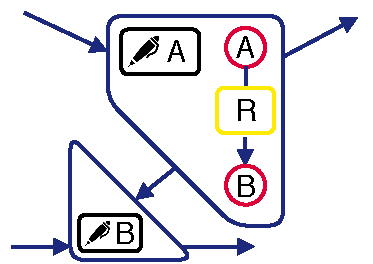
\includegraphics[width=.7\linewidth]{xchange/assets/trustchain_tutorial_4}
		\caption{To improve scalability, we extend the TrustChain structure to support concurrent block creation.}
		\label{fig:trustchain_tutorial_4}
	\end{subfigure}\hspace{0.05\textwidth}%
	\begin{subfigure}[t]{.33\textwidth}
		\centering
		\captionsetup{width=\linewidth}
		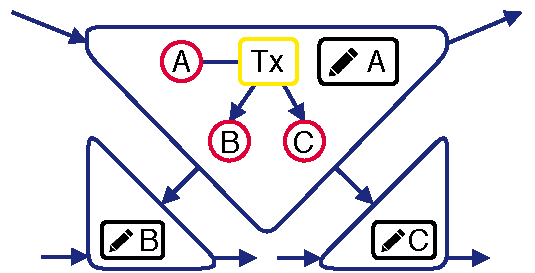
\includegraphics[width=\linewidth]{xchange/assets/trustchain_tutorial_5}
		\caption{By extending the number of pointers and signatures, we add support for multi-party agreements.}
		\label{fig:trustchain_tutorial_5}
	\end{subfigure}
	\caption{Recording transactions in TrustChain.}
	\label{fig:trustchain_tutorial}
\end{figure*}

We argue that TrustChain is a suitable blockchain to use during the \ModelName{} trading protocol for the following five reasons.
%We identify five major advantages of TrustChain over other distributed ledgers that motivate usage of TrustChain during the \ModelName{} protocol. % is a suitable distributed ledger for \ModelName{} for the following five reasons.
First, it is a blockchain that is optimized for efficient and tamper-proof accounting of generic data items within transactions.
The accounting capabilities of TrustChain enable \ModelName{} to securely persist trade specifications.
Second, TrustChain does not require network-wide replication of all transactions but enables individuals to selectively share parts of their individual ledger with others.
This highly reduces storage requirements and allows \ModelName{} to also run on devices with storage limitations.
Third, TrustChain does not require any trusted authority for the creation, validation, or storage of transactions.
This satisfies our requirement for decentralization, avoiding any reliance on trusted third parties during the \ModelName{} trading protocol.
Forth, the TrustChain structure is optimized for bilateral interactions that are signed by two parties but also supports the creation of unilateral transactions.
This aligns well with the \ModelName{} trading protocol since several operations benefit from support for bilateral transactions (e.g., trade agreements).
Finally, TrustChain is already being used by various decentralized applications that require scalable accounting~\cite{pouwelse2017laws}.
At the time of writing, the global TrustChain ledger contains over 64 million transactions, created by 41.098 unique identities.\footnote{http://explorer.tribler.org}

%We emphasize that \ModelName{} can be built on \emph{any} distributed ledger with accounting capabilities.
%Our proposed trading protocol in Section \ref{sec:xchange_protocol} can leverage other distributed ledger technologies besides TrustChain.
%However, depending on the specifications of the ledger being used this could introduce the inefficiencies that we specifically try to avoid.

\subsection{Recording TrustChain Transactions}
We now outline how a transaction between two interacting users $ A $ and $ B $ is recorded in TrustChain, see Figure \ref{fig:trustchain_tutorial}.
Figure \ref{fig:trustchain_tutorial_1} highlights one block containing a transaction between $ A $ and $ B $.
Each block contains a single transaction (\emph{Tx}).
A transaction is a generic description of any interaction between users, for instance, making an agreement or recording a trade.
%We consider a transaction to be the result of \emph{any} interaction between users, like transferring assets or recording agreements. %We intentionally consider a transaction to be a description of any interaction between two users.
% As a result, it can describe almost every interaction between two or more users, like asset transfers or generic agreements.
Both transacting parties digitally sign the transaction they are involved in by using any secure digital signing algorithm.
These signatures are included in the block and ensure that participation by both parties is irrefutable.
It also confirms that both parties agree with the transaction itself.
Digital signatures can be effectively verified by others.
After all required signatures have been added to a record, the transaction is committed to the local databases of the two interacting parties.
%Each transaction has a \emph{type} field, indicating its purpose.
%Blocks are linked together by a (hash) pointer that points to the prior block in each individual ledger.
%Both transacting parties digitally sign the transaction they are involved in by using any secure digital signing algorithm (TrustChain uses the ECDSA algorithm).
%These digital signatures are included in a block, which ensures that participation by both parties is irrefutable.
%It also confirms that both parties agree with the content within the transaction.
%Others can efficiently verify digital signatures in blocks since the digital identities of both interacting parties (their public keys) are also included in a block.
%After all required signatures have been added to a block, the block is appended to the individual ledgers of the two interacting parties and committed to their local databases.
%TrustChain also allows unilateral transactions without any counterparty.
%The block with a unilateral transaction is only signed by the issuing party and then committed to their individual ledger.

The security of stored blocks is improved by linking them together, incrementally ordered by creation time.
In particular, each block is extended with a description (hash) of the prior block.
Each block has a sequence number that indicates its position in the individual ledger.
This yields the blockchain structure as shown in Figure \ref{fig:trustchain_tutorial_2}.
%The hash of each block can be effectively computed with any cryptographically secure hashing algorithm (our implementation uses SHA256).
As a result, each user maintains their own local chain which contains all transactions in which they have participated.
This sets TrustChain apart from the structure of traditional blockchains, where the entire network maintains a single, linear ledger.

Note how the blockchain structure in Figure \ref{fig:trustchain_tutorial_2} allows user $ A $ to modify blocks in their individual ledger without being detected by others.
In particular, $ A $ can reorder the blocks in its individual ledger since validity can quickly be restored by recomputing all hashes.
In most blockchain applications, the global consensus mechanism prevents this kind of manipulation.
TrustChain uses a more efficient approach: each block is extended with an additional (hash) pointer that points to the prior block in the individual ledger of the transaction counterparty.
This is visualized in Figure \ref{fig:trustchain_tutorial_3}.
Each block now has exactly two incoming and two outgoing (hash) pointers, except for the last block in an individual ledger, which only has two incoming pointers.
Modifications of the individual ledger by $ A $, like reordering or removing blocks, can now be detected by a transaction counterparty.
To prove this fraud, the transaction counterparty reveals both the correct block and the invalid block created by $ A $.

When two parties transact and create a block, their chains essentially become entangled.
%This property makes fraud impractical to hide since a counterparty is able to proof malicious activities by revealing his block with the disputed transaction.
When users initiate more transactions with others, it leads to the directed acyclic graph (DAG) structure as shown in Figure \ref{fig:trustchain}.
Figure \ref{fig:trustchain} shows seven blocks, created by seven unique users.
%For clarity, the figure hides digital signatures in a block.
Each block is added to the local chains of all parties involved in the transaction exactly once.
For a more advanced analysis of the technical specifications and security of TrustChain, we refer the reader to the original paper by Otte et al.~\cite{otte2017trustchain}.

\begin{figure}[t]
	\centering
	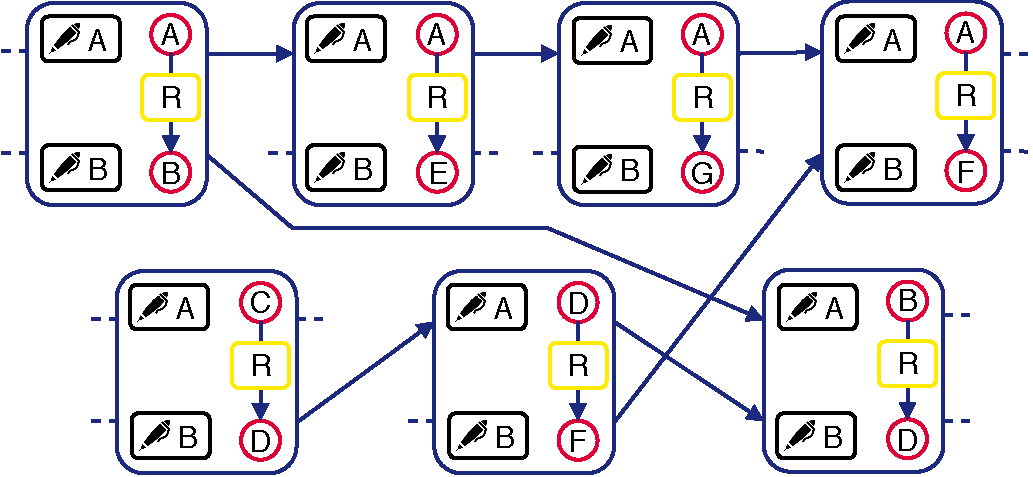
\includegraphics[width=.8\linewidth]{xchange/assets/trustchain}
	\caption{The TrustChain ledger, with seven blocks created by seven participants.}
	\label{fig:trustchain}
\end{figure}

\subsection{Improving TrustChain Scalability}
According to Otte et al., TrustChain is designed to scale~\cite{otte2017trustchain}.
However, we identify that its design limits a user to one pending block creation at once.
The main issue is that the digital signature of the transaction counterparty is required before a new block can be appended to an individual ledger (since the input for the hash of each new block includes all signatures in the previous block).
This enables an attack where a malicious user can purposefully slow down the block creation of others by delaying the signing process of a bilateral transaction it is involved in.
It also limits the growth rate of individual ledgers and reduces the overall scalability of TrustChain.

We contribute to TrustChain and improve its scalability by adding support for \emph{concurrent block creation}.
The idea is to remove the requirement for a digital signature of the counterparty when appending new blocks to an individual ledger.
We believe that this concurrency is necessary since it allows traders to engage in transactions with different parties while being engaged in a trade.

Our solution is visualized in Figure \ref{fig:trustchain_tutorial_4}.
It shows a transaction between users $ A $ and $ B $, initiated by $ A $.
We partition a block in two parts, and each block partition is appended to the individual ledger of exactly one party.
Construction of a block between $ A $ and $ B $ now proceeds as follows: first, user $ A $ initiates a transaction by constructing a block partition with the transaction content and its digital signature.
User $ A $ adds this block partition to its individual ledger immediately (note that it does not include the digital signature of $ B $).
$ A $ now sends the block partition to $ B $.
If $ B $ agrees with the transaction, it signs the block partition created by $ A $, adds it to its individual ledger and sends his block partition (with their signature) back to $ A $.
User $ A $ stores the block partition created by $ B $ in its local database.
Participation of both parties in this transaction can now be proven with both block partitions.
This mechanism allows users to be involved in multiple transactions and block constructions at once.

We further improve upon the TrustChain design and enable support for multi-party agreement, see Figure \ref{fig:trustchain_tutorial_5}.
By extending the number of pointers and signatures, we can securely record transactions between more than two parties.
Block partitions can now be represented as a tree, where the root node is the block partition created by the transaction initiator.
While we do not currently use this mechanism in \ModelName{}, we believe this allows for more advance features like support for $n$-way trades~\cite{wang2018loopring}.

\subsection{Storing Trade Specifications on TrustChain}
We now outline how trade specifications are stored within transactions on TrustChain.
Figure \ref{fig:trustchain_market} shows a part of the TrustChain ledgers of traders $ A $ and $ B $.
It includes a sequence of transactions that indicate a finished trade between $ A $ and $ B $.
Trade agreements, created during phase III in the \ModelName{} trading protocol, are stored within a bilateral \TRAgreement{} transaction which is digitally signed by both involved traders.
Individual payments are stored within bilateral \TRPayment{} transactions.
A \TRPayment{} transaction that indicates an asset transfer from trader $ A $ to $ B $ is only signed by $ A $ if the assets are successfully transferred, and only signed by $ B $ if the assets are observed in one of their wallets.
Finally, trade finalizations are stored within bilateral \TRTradeDone{} transactions.

\begin{figure}[t]
	\centering
	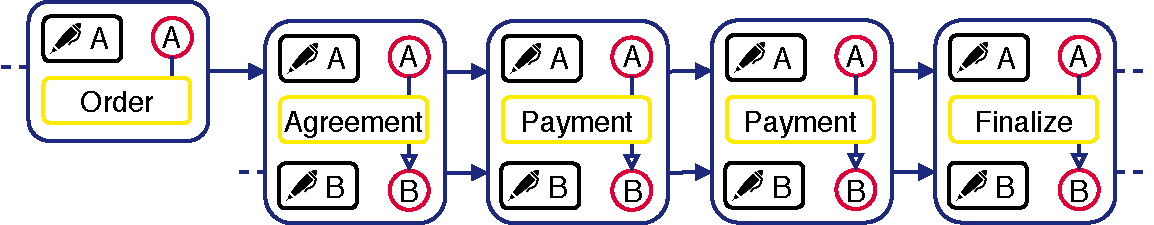
\includegraphics[width=\linewidth]{xchange/assets/trustchain_market}
	\caption{A part of the TrustChain ledger, storing an offer and request created by traders $ A $ and $ B $ respectively, and full specifications of a finished trade between $ A $ and $ B $.}
	\label{fig:trustchain_market}
\end{figure}

Since the overhead of creating new TrustChain transactions is low, we also store offers and requests as unilateral transactions.
Figure~\ref{fig:trustchain_market} shows a \TROffer{} transaction, created by user $ A $, and a \TRRequest{} transaction, created by user $ B $.
Each of these transactions only contain a digital signature of its creator.
%New orders are stored on TrustChain within unilateral transactions.
%These transactions only contain the digital signature of the peer that created the transaction.
Note that new orders stored on individual ledger of a specific peer are not locked in time until this peer initiates a bilateral transaction with another peer.



%\section{Counterparty Fraud Analysis}
%\label{sec:security}
%We now analyse the effectiveness of counterparty fraud conducted by an adversary $ A $.
%Recall that the goal of our adversary is to conduct counterparty fraud and compromise assets from other traders.
%Our first observation is that $ A $ is unable to interfere in the asset exchange between two other traders, say $ B $ and $ C $.
%In particular, trade between $ B $ and $ C $ only involves these two traders and settlement providers.
%As such, the adversary is unable to conduct counterparty fraud during their trade without control over the settlement providers, which we have assumed to be trusted parties.

%If our adversary $ A $ aims to conduct counterparty fraud, it must be engaged in a trade with another party, say $ D $.
%Recall that the trader initiating the first asset transfer takes some risk since it is uncertain whether the counterparty will fulfil its obligations and transfer assets back.
%If the first asset transfer moves assets from $ D $ to $ A $, $ A $ can disconnect from the network after having received assets from $ D $.
%Note here that incremental settlement limits the effectiveness of this fraud to $ \frac{1}{n} $ of the total value exchange (where $ n $ is the total number of asset transfer operations initiated by $ D $).
%If $ A $ would disconnect after receiving assets from $ D $, it has successfully conducted counterparty fraud and compromised assets.

%Our adversary $ A $ now wants to engage in a trade with another trader $ E $ and conduct counterparty fraud with them.
%During the trade negotiation phase between $ A $ and $ E $, $ E $ would detect the pending asset exchange between $ A $ and $ D $ by inspection of the individual ledger of $ A $ (also see step 4 in Section \ref{sec:xchange_protocol}).
%As such, $ E $ refuses to trade with $ A $ until $ A $ and $ D $ completed their trade, and $ A $ is only able to conduct counterparty fraud with a single trading partner.
%This property significantly reduces the possibility of $ A $ to conduct counterparty fraud with multiple trading partners in \ModelName{}.

%We should note that $ A $ can prevent a trading partner $ E $ from trading with others by purposefully delaying the settlement process.
%To address this, we propose a minor modification to the trading protocol where a trader only refuses to trade with the counterparty that has an asset transfer operation pending to another trading partner.
%This can be detected when a reference to a publicly available transaction is included in a \texttt{Payment} block.
%How to detect pending asset transfers when the asset ecosystem cannot be queried by other traders, remains an open research question.


\section{Implementation and Evaluation}
\label{sec:evaluation}
%We have implemented the \ModelName{} architecture and protocol in the Python 2.7 programming language, and published its code on GitHub\footnote{Can be requested through the Program Chair.}.
We present the open-source implementation of \ModelName{} and an experimental evaluation.
The evaluation answers the following three questions: (1) what is the duration of a single trade when \ModelName{} is deployed on low-resource devices? (2) How scalable is \ModelName{} in terms of throughput and bandwidth usage when increasing the system load? And (3) how does the scalability of \ModelName{} compare with that of state-of-the-art decentralized asset exchanges?

\subsection{Implementation Details}
\label{sec:implementation}
We have implemented the \ModelName{} trading protocol and system architecture in the Python 3 programming language.
%Our implementation spans a total of 4.702 lines of code.
%This number excludes any source code related to the unit tests.
%The correctness of the code is verified by 213 unit tests, covering 92\% of the code in the \emph{core} package (which contains the overlay logic and most of the components in the \ModelName{} system architecture).
The implementation is open source and all software artifacts (source code, tests, and documentation) are published on GitHub.\footnote{https://github.com/tribler/anydex-core}

\textbf{Networking.}
We have built \ModelName{} on top of an existing networking library
%Since TrustChain is built upon the IPv8 decentralized networking library, we decided to adopt it for all network communication generated by \ModelName{}.
%Our motivation for this is that TrustChain utilizes the same networking library.
which provides the functionality to devise decentralized overlay networks and has built-in support for authenticated network communication, custom message definitions, and UDP hole punching.\footnote{https://github.com/tribler/py-ipv8}
For efficiency reasons, the UDP protocol is used for message exchange between peers.
The \ModelName{} implementation uses request stores to handle message timeouts and transmission errors.
%It requires no central server to run, except for bootstrapping in the live network.
%Our implementation of \ModelName{} defines 15 distinct types of network messages, of which 11 are used to notify traders about matched orders and to manage execution of trade.

\textbf{Architecture.}
We have implemented all components of the \ModelName{} system architecture, presented in Figure~\ref{fig:mechanism_architecture}.
Request stores are organized in a dictionary with the request identifiers as keys and the individual request stores as values.
The matching priority queue is implemented as a linked list that remains sorted whenever new entries are added to it.
Different order books are organized in a dictionary whose keys are an asset pair, and the values are the individual order books.
We provide both an implementation of a basic order book and an implementation of a limit order book.
The basic order book structure can be used to store and match orders with any attributes.
The limit order book is optimized to store asset trading orders with pricing information and organizes orders with the same price in a so-called \emph{price level}.
It traverses through the set of orders based on these price levels during order matching.
%The timeout for \texttt{ProposeTrade} messages, $ T_p $, is fixed to five seconds, which is well above measured Internet round-trip times~\cite{Acharya1998ASO}.
%This value should be increased when MATCH is deployed in networks with higher round-trip times.

\textbf{Wallets.}
Our implementation contains a \texttt{Wallet} base class that can be extended by programmers to create wallets that store different types of assets.
For testing purposes, we have implemented a \texttt{DummyWallet}, which is used when executing the unit tests and when running our experiments.
This wallet does not interact with any settlement provider.
For practical reasons, we also provide a \texttt{BitcoinWallet} that invokes the \emph{bitcoinlib} library to query Bitcoin balance or to transfer Bitcoin to other wallets.\footnote{http://github.com/1200wd/bitcoinlib}
This library communicates with full nodes operating in the Bitcoin network.

\textbf{Policies.}
The implementation contains base classes for the different policies that \ModelName{} requires.
Developers can implement their own advanced policies by subclassing these base classes.
For example, programmers can add custom matching policies by subclassing the \texttt{MatchPolicy} class and by providing an implementation of the \texttt{match(order, order\_book)} method.
This method accepts the order being matched and an order book as parameters and returns a list of orders that matches the passed order.
We provide an implementation of the \emph{price-time} matching policy.
This policy is used when matching assets that contain a price expressed in terms of another asset.
%It matches orders first based on price, and then on time since order creation, while prioritizing orders that have been open for a longer time.
The experiments in this section use this matching policy to match new orders.
We implement and use a basic validation policy that checks whether an incoming order has not expired yet.
Finally, we provide a basic order dissemination policy where a new order is sent to the same subset of matchmakers every time.

\subsection{Trading on Low-resource Devices}
\label{sec:exp_trading_low_devices}
The first experiment determines the total duration of a trade between two traders when running \ModelName{} on low-resource devices.

\textbf{Setup.}
This experiment is conducted with two hosted Raspberry Pis (3rd generation, model B+).
The devices run the Raspbian Stretch operating system and the Python 3.5 interpreter.
Each device creates an order, and the two created orders indicate mutual interest in a trade.
One device assumes the identity of trader $ A $ and the other device acts as trader $ B $.
To avoid the transmission of redundant \MsgMatch{} messages, only one of the two devices acts as a matchmaker.
The experiment is executed in an isolated environment: there is only network communication between the two Raspberry Pis.
For this experiment, we use two different subclasses of \emph{DummyWallet}.
We configure these wallet such that assets instantly arrive when being transferred to another wallet.
We do so to measure the overhead of \ModelName{} itself, and not that of asset transfer operations.

During the experiment, we log the timestamp of several events. %, such as the creation of new orders, the transmission of trade proposals and acceptance of trade proposals.
At $ t=0 $, both orders are created.
The trade is finished when both trading parties have signed a \TRTradeDone{} transaction and have committed the transaction to their individual ledgers.

\begin{figure}[t]
	\centering
	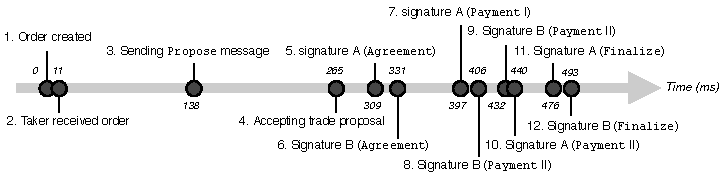
\includegraphics[width=\linewidth]{xchange/assets/trade_timeline}
	\caption{A timeline of the events during a single trade between two traders $ A $ and $ B $. The experiment is conducted on two hosted Raspberry Pis (3rd generation, model B+). The total duration of the trade is 493 milliseconds.}
	\label{fig:trade_timeline}
\end{figure}

\textbf{Results.}
Figure \ref{fig:trade_timeline} shows a timeline of the events during a single trade between the two Raspberry Pis.
The full trade sequence, from the moment of order creation to mutual possession of a dual-signed \TRTradeDone{} transaction, completes in 493 milliseconds, less than half a second.
Almost half of the trade duration, 254 milliseconds, is spent in phase III of the \ModelName{} trading protocol, the trade negotiation phase.
During this phase, a trader determines whether a matched counterparty is already involved in a trade by inspection of the entries in their TrustChain ledger.
Note that at the start of the trade negotiations, both traders have a single transaction in their individual TrustChain ledger, containing specification of their created order.
%These blocks are then exchanged during ledger inspection by the counterparty.

\textbf{Conclusion.}
This experiment shows that a full trade, including order creation, can be completed within half a second on low-resource devices if asset transfer would be instant.
Since orders are published as unilateral transactions on TrustChain, order creation is almost instant.
This duration is significantly lower than the block creation times of state-of-the-art DEXes.
For example, the average block creation time of the NEM blockchain platform is around 60 seconds on average~\cite{nem2018nem}.
This means that it can take up to a minute before a new order is confirmed on the NEM blockchain.

An implementation of \ModelName{} in a real Internet-of-Things environment would be viable since its communication and transaction creation overhead is minimal compared to existing decentralized asset trading marketplaces (see Section~\ref{subsec:scalability_experiment}).
However, our trading protocol requires periodic queries of other blockchain ledgers during an ongoing trade.
Since maintaining the full transaction history is not realistic given the storage restrictions of IoT devices, \ModelName{} should rely on dedicated full nodes that maintain synchronized with all transactions on a specific blockchain.
We believe that devices with less processing capabilities than the Raspberry Pis used during this experiment are capable of maintaining and securing individual TrustChain ledgers.
This should be verified with a small-scale deployment of \ModelName{} in an IoT environment where blockchain-based assets are managed.

While the low trade duration on low-resource devices is a promising result, the experiment is not representative of a realistic trading environment where there are many traders creating orders and exchanging assets simultaneously.
Therefore, our next experiment focuses on the scalability of \ModelName{} and reveals how our mechanism behaves under a higher system load.

\subsection{Scalability of \ModelName{}}
\label{subsec:scalability_experiment}
We now perform scalability experiments to quantity the performance of \ModelName{} as the system load and network size increases.

\textbf{Setup.}
To explore the limitations of \ModelName{}, we conduct scalability experiments on our university cluster.
The detailed specifications of the hardware and runtime environment can be found online.\footnote{https://www.cs.vu.nl/das5/}
Our infrastructure allows us to reserve computing nodes and deploy instances of \ModelName{} on each node.
We use the Gumby experiment framework to orchestrate the deployment of \ModelName{} instances onto computing nodes and to extract results from experiment artifacts.\footnote{https://github.com/tribler/gumby}
The scalability experiment is controlled by a \emph{scenario file}, a chronologically ordered list of actions which are executed by all or by a subset of running instances, at specific points in time after the experiment starts.
Each run is performed at least five times, and the results are averaged.

We increase the system load, namely the number of new orders being created every second.
As the system load grows, so does the number of traders in the network.
With a system load of $ l $ new orders per second, we deploy $ 0.5l $ \ModelName{} instances.
We devise a synthetic dataset to determine the performance of \ModelName{} under a predictable arrival rate of orders.
In a network with $ n $ peers running \ModelName{}, $ n $ orders are created every half a second.
Each peer alternates between the creation of an offer and a request.
To avoid the situation where all instances create new orders at the same time, the starting time of this periodic order creation is uniformly distributed over all peers, based on their assigned IDs (ranging from 1 to $ n $).
Each peer acts as a matchmaker and sends a new order to four matchmakers, which each peer randomly selects when the experiment starts.
The experiment lasts for 30 seconds, after which $ 60n $ orders are created in total.
We fix the price of each new offer and request to \$1 and the asset quantities to 1, to make matchmaking a predictable process.
After 30 seconds, the experiment is terminated.

We test the scalability of \ModelName{} under a combination of different risk mitigation strategies.
The $ RESTRICT(t) $ policy denotes the policy where a trader will not trade with a counterparty that currently holds responsibility in $ t $ or more ongoing trades (see Section \ref{sec:limit_risk}).
With the $ INC\_SET(n) $ policy, we refer to the incremental settlement strategy where each trader makes $ n $ payments to the counterparty during a single trade.
We consider four experiment settings in total, with combinations of the $ RESTRICT(1) $ and $ INC\_SET(2) $ policies, and when no risk mitigation policy is active.
Scalability is measured as follows:
first, we analyse the peak \emph{throughput} observed during the experiment, in terms of trades per second.
Second, we consider the average order fulfil \emph{latency}, which is the time between the creation of an order and the time until this order has been completed (the order creator has exchanged all assets as specified in the order).

\begin{figure*}[t]
	\centering
	\begin{subfigure}[t]{.5\textwidth}
		\centering
		\captionsetup{width=.9\linewidth}
		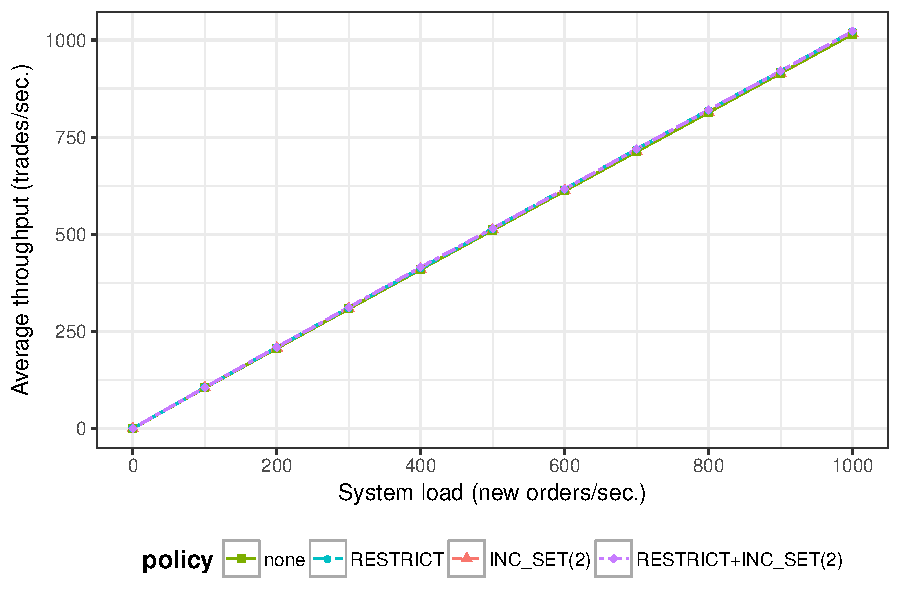
\includegraphics[width=.95\linewidth]{xchange/assets/experiments/scalability}
		\caption{Peak throughput}
		\label{fig:scalability}
	\end{subfigure}%
	\begin{subfigure}[t]{.5\textwidth}
		\centering
		\captionsetup{width=.9\linewidth}
		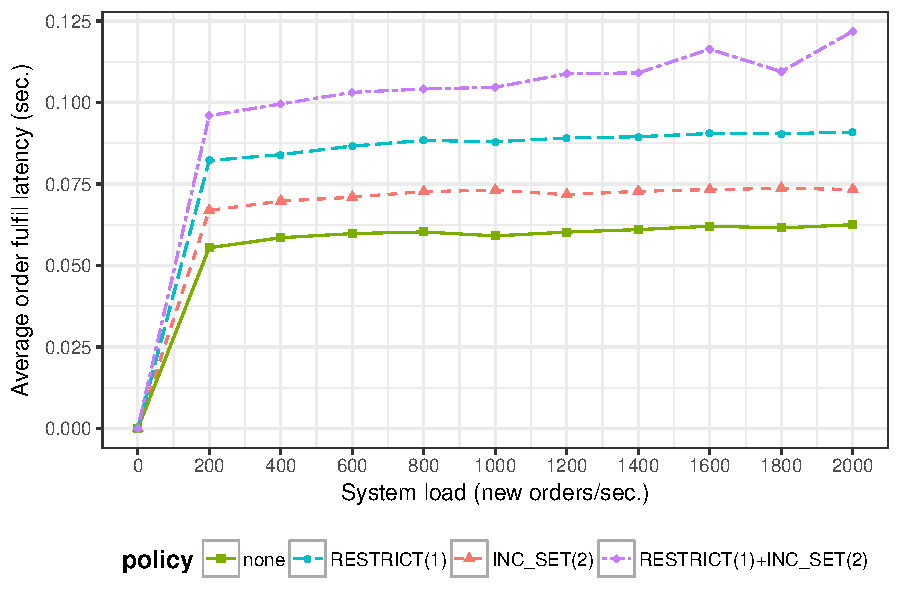
\includegraphics[width=.95\linewidth]{xchange/assets/experiments/latency}
		\caption{Average order fulfil latency}
		\label{fig:latency}
	\end{subfigure}%
	\caption{The peak throughput and order fulfil latencies as the system load increases.}
	\label{fig:scalability_latency}
\end{figure*}

%We consider three different (clearing) policies.
%The \texttt{NOCHECK} policy does not verify whether a counterparty holds responsibility for any trade it is engaged in, i.e., the content of their ledger is not inspected during trade negotiation.
%This means that a trader can be involved in trade with an unlimited number of counterparties at the same time under this policy.
%With the \texttt{CHECK} policy active, a trader will check a counterparty during trade negotiation but it will not refuse to trade if the counterparty holds responsibility in an ongoing trade.
%The \texttt{CHECK+LIMTRADE} both checks a counterparty during trade negotiation and refuses to trade if the counterparty is already involved in a trade (this is the default policy that \ModelName{} adopts).
%Although the \texttt{NOCHECK} and \texttt{CHECK} policies do not limit counterparty fraud, a separate evaluation of these policies helps to understand the impact of inspecting the distributed ledger of trading counterparties during the negotiation phase.

\textbf{Results.}
The results of the scalability experiments are presented in Figure~\ref{fig:scalability_latency}.
We run each experiment with a specific system load up to 1.000 deployed instances (which is close to the limitations of the used hardware).
Figure~\ref{fig:scalability} shows how the peak throughput (expressed in trades per second, vertical axis) behaves with respect to the system load (horizontal axis).
All experiment settings hint at linear scalability as the system load increases.
Furthermore, enabling risk mitigation policies does not appear to have a notable effect on the peak throughput.
Experimentation on more compute nodes should reveal whether this trend continues when the system load exceeds 2.000 new orders per second.
%However, when the network size increases beyond 300 deployed instances, the throughput increase slows down for the \texttt{CHECK} and \texttt{CHECK+LIMTRADE} policies.
%We explain this as follows: when the network size increases, more trades are being made, resulting in more transactions in each individual ledger.
%Since more TrustChain blocks have to be exchanged and verified during the trade negotiation phase, it takes longer before a trader sends out a trade proposal, or accepts an incoming trade proposal.

Figure~\ref{fig:latency} shows the average order fulfil latency when the system load increases, for the four evaluated experiment settings.
The average order fulfil latency remains largely constant when the system load grows.
Applying the restriction and incremental settlement policies increases the average order fulfil latency, since more operations have to be performed to successfully complete an order.
We observe that there is a moderate increase of latency when applying the $ RESTRICT(1) + INC\_SET(2) $ policies when the system load grows to 2.000 trades per second.
The high system load is likely to increase the duration of individual trades beyond 0.5 seconds, which means that the $ RESTRICT(1) $ policy prevents traders from initiating a new trade with others.
Since a trader now has to find a new party to trade with, the average order fulfil latency increases.

%The average bandwidth usage under the \texttt{NOCHECK} policy remains constant when the network consists of more traders.
%When checking the ledgers of counterparties during trade negotiation, bandwidth usage increases significantly and grows roughly linear as the network size increases.
%Even when running the experiment with only 50 XChange instances, the total bandwidth usage increases by a factor 11, compared to the \texttt{NOCHECK} policy.
%Further inspection reveals that this bandwidth increase is indeed caused by the overhead of requesting TrustChain transactions from counterparties.

\textbf{Conclusion.}
The main finding of this experiment is that the throughput (trades per second) scales linearly with respect to the system load and network size.
We also observe that the average order fulfil latency remains largely constant as the system load grows.
Further experimentation should reveal whether these trends continue with a higher order creation rate.

\subsection{Scalability comparison}
\label{sec:experiment_comparison}
%We compare the scalability of \ModelName{} with related systems in the domain of decentralized asset trading.
We compare the scalability of \ModelName{} with that of state-of-the-art DEXes.
This work is the first to present a systematic scalability comparison between DEXes, to the best knowledge of the authors.
For the following experiment, we compare \ModelName{} with the BitShares and Waves DEXes respectively.
BitShares and Waves have attained significant market capitalization (\$80 million and \$83 million respectively), and have employed consensus mechanisms that are fundamentally different compared to the TrustChain blockchain used by \ModelName{}.
We briefly discuss BitShares and Waves.

\textbf{BitShares.}
BitShares enables users to issue, manage and trade their own assets, which are stored on a single blockchain~\cite{schuh2015bitshares}.
%The BitShares decentralized exchange is build upon the Graphene open-source blockchain.
To coordinate block creation, BitShares uses the Delegated Proof-of-Stake (DPoS) consensus mechanism~\cite{larimer2014delegated}.
DPoS utilizes approval voting to decide on a committee of so-called \emph{witnesses}.
Witnesses are able to append a new block to the blockchain (produce a block), in a round-robin fashion, and are rewarded by the sum of transaction fees in a block they have added to the ledger.
If a witness acts malicious, i.e. by deliberately failing to produce a new block, the witness will eventually be removed from the committee by stakeholders.
%The developers of BitShares claim a theoretical throughput of 100.000 transactions per second on a single machine.
%Their analysis however, does not consider limitations incurred by message exchange in peer-to-peer network, which 
All orders are stored on the BitShares blockchain.
Matching of orders proceeds by a deterministic algorithm during transaction validation.
Specifications on resulting matches are not stored on the blockchain, to improve efficiency (but they can be deduced by replaying transactions).
%They can be reconstructed by users that  % are able to replay the blockchain and determine how orders were matched.

We compile BitShares version 3.3.2.
During our experiments, we deploy a committee with 21 witnesses that produce blocks, comparable to the committee in the BitShares mainnet at the time of writing.
We fix the block creation interval to five seconds.

\textbf{Waves.}
Similar to BitShares, the Waves platform also allow users to create and manage custom assets~\cite{wavesplatform}.
%Waves was proposed in earlier 2016 and launched in November 2016.
The adopted consensus mechanism is Waves-NG, a protocol that combines Proof-of-Stake and Bitcoin-NG~\cite{eyal2016bitcoin}.
%According to their website, Waves-NG is capable of supporting 42 transactions per second.
%Users are also able to 'lease' stake to miners in the network and receiving rewards proportional to their invested stake.
Although the blockchain in Waves is a decentralized data structure, order matchmaking in Waves is largely centralized and traders submit new orders to a single matchmaking instance.
The submitted order can then only be matched with other orders this matchmaker knows about.
When two orders are matched by a matchmaker in Waves, the resulting assets are exchanged on the blockchain and this trade is then recorded as a transaction.
The matchmaker collects the transaction fees in both matched orders.

We compile Waves version 1.1.5 and adopt all default settings when deploying a Waves development network.
%Waves is configured to use a base target of 100, the default setting when creating a private testnet.
To ensure a relatively quick block creation, the average time between creation of two blocks is lowered to five seconds.
We configure each deployed Waves instance to run a matchmaker.
Each Waves instance sends new orders to another Waves instance, which remains fixed throughput the experiment.

\textbf{Setup.}
Similar to the prior experiment, we increase the system load and observe the peak throughput and average order fulfil latency of each system.
%For each run with XChange, BitShares and Waves, we increase the system load, or the number of new orders per second.
For each run with BitShares or Waves, we initiate the experiment by starting a single BitShares/Waves instance, which creates two new types of digital assets on the blockchain.
This instance then transfers sufficient assets to all other instances, so they can create new orders and trade these assets with others.
%After five seconds, we start the other $ n - 1 $ instances which then connect to the first instance.
When each instance has sufficient funds to create numerous orders, they start to create a new order every half a second, for one minute in total.
We adopt the same synthetic workload as in the previous scalability experiment.
For \ModelName{}, we enable the $ RESTRICT(1) $ and $ INC\_SET(2) $ risk mitigation policies.
%We use the synthetic workload described in Section \ref{subsec:dataset} and subject each of the implementations to exactly the same trading workload.
%Instances create orders during a period of five minutes.
%Each run during this experiment is executed once.

%We define the maximum transaction throughput observed during each run as our scalability metric. %, or transactions
%When the experiment ends, we determine the peak throughput, expressed in transactions per second.
In the prior experiments, we have adopted the peak number of trader per second as our scalability metric.
In order to fairly compare the scalability between \ModelName{}, BitShares, and Waves, we modify the throughput metric and quantify the peak number of \emph{operations} per second observed during the experiment.
%Since there is no standardized way to compare throughput between the tested systems, we first have to define what we consider as a transaction.
For BitShares, we count the number of operations included in a transaction.
For Waves, we consider a new transaction on the blockchain as a single operation. % that are the result of two orders matched by a matchmaker.
For XChange, we consider the creation of a block in an individual ledger as a single operation. % and determine the second during which the most of such blocks are created.

\begin{figure*}[t]
	\centering
	\begin{subfigure}[t]{.5\textwidth}
		\centering
		\captionsetup{width=.9\linewidth}
		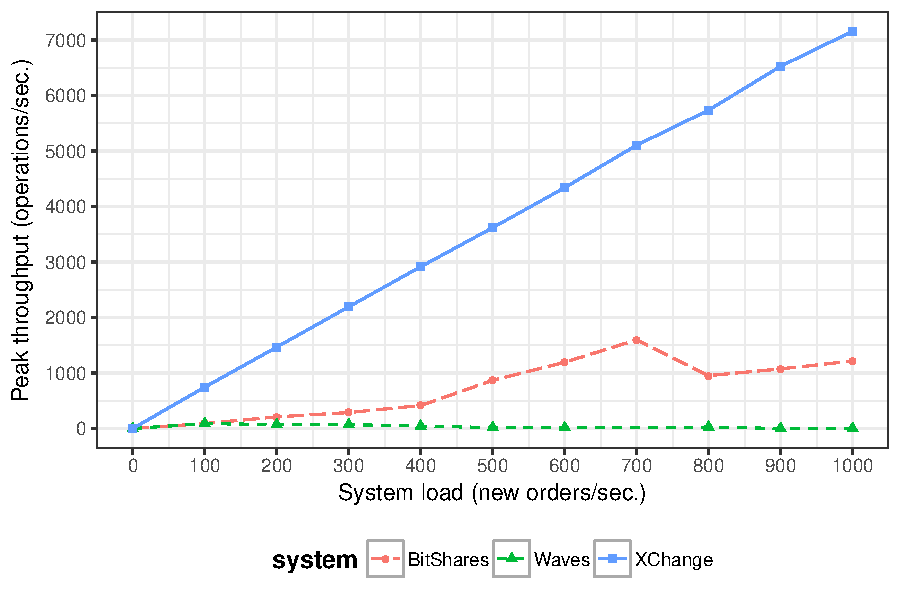
\includegraphics[width=.95\linewidth]{xchange/assets/experiments/scalability_comparison}
		\caption{Peak throughput}
		\label{fig:scalability_comparison}
	\end{subfigure}%
	\begin{subfigure}[t]{.5\textwidth}
		\centering
		\captionsetup{width=.9\linewidth}
		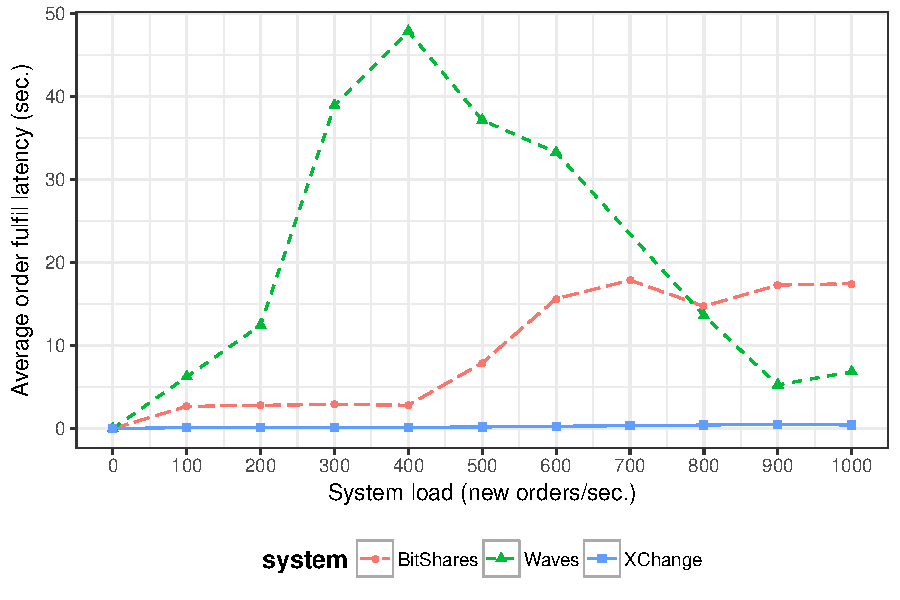
\includegraphics[width=.95\linewidth]{xchange/assets/experiments/latency_comparison}
		\caption{Average order fulfil latency}
		\label{fig:latency_comparison}
	\end{subfigure}%
	\caption{The peak throughput and order fulfil latencies of \ModelName{}, BitShares and Waves, as the system load increases.}
	\label{fig:scalability_latency_comparison}
\end{figure*}

\textbf{Results.}
Figure~\ref{fig:scalability_latency_comparison} shows the scalability of \ModelName{}, BitShares and Waves.
Figure~\ref{fig:scalability_comparison} shows how the peak throughput in terms of operations per second behaves as the system load increases.
The peak throughput of Waves does not exceed 89 operations per second.
Furthermore, we observe that a majority of the deployed Waves instances crashes due to memory limitations when increasing the system load to 300 new orders per second.
The consensus mechanism of Waves is not able to keep up with the increasing system load.
Up to a system load of 400 new orders per second, BitShares shows a linear increase in peak throughput.
Surprisingly, when the system load exceeds 400 new orders per second, peak throughput grows faster.
We found that BitShares has issues keeping up with a higher load, and the inclusion of orders in the BitShares blockchain might be deferred.
Even though the system load is predictable throughout the experiment, the number of transactions inside new blocks on the BitShares blockchain becomes more uneven when the system load grows.
Figure~\ref{fig:scalability_comparison} reveals that \ModelName{} exhibits a near-linear increase in peak throughput.
The TrustChain ledger as used by \ModelName{} achieves the creation of 7.000 new blocks (operations) per second.

Figure~\ref{fig:latency_comparison} shows the average order fulfil latency of \ModelName{}, BitShares and Waves as the system load increases.
The order fulfil latency of Waves increases up to almost 48 seconds, and then starts to decline.
Up to a system load of 400 new orders per second, BitShares shows an average order fulfil latency of around 2.5 seconds.
This is expected since the block creation interval is fixed to five seconds and on average, it takes 2.5 seconds for a new order to be fulfilled.
When the system load grows, so does the average order latency, confirming our finding that the inclusion of incoming orders in a block becomes a less predictable process.
Finally, note how the average order fulfil latency of \ModelName{} remains sub-second during this experiment.

\textbf{Conclusion.}
\ModelName{}, in combination with the TrustChain ledger, shows excellent scalability compared to the BitShares and Waves DEXes.
At this point, we should note that TrustChain, unlike BitShares and Waves, does not incorporate global consensus and therefore has different security guarantees.
Also, during this experiment we assume that \ModelName{} assets are exchanged instantly between trading parties, which is done to quantify the limitations of \ModelName{}.
In reality, a trader most likely has to wait one or more block creation intervals in order to guarantee that a payment is finalized.
This further adds to the order fulfil latency.

%We note that the current implementation of \ModelName{} queries all transactions that a peer does not have in its local TrustChain database during trade negotiation.
%This process causes significant bandwidth overhead (as revealed by Figure~\ref{fig:bandwidth_usage}) and adds latency before a trade proposal is accepted or rejected.
%We propose two optimizations to address this issue.
%The first optimization is to store more information in each transaction created during the XChange protocol, e.g., a pointer to an ongoing trade.
%This highly reduces the number of transactions that each trader requires during the \ModelName{} trading protocol, at the cost of a marginal increase in storage requirements.
%The second optimization is to periodically request blocks from random traders while not being involved in a trade and to verify them.
%The rate at which new blocks are requested from others can be adapted to match the hardware specifications of the device that runs \ModelName{}.
%We leave these optimizations and an analysis of their impact on performance as further work.

%\begin{table*}[t]
%	\small
%	\centering
%	\begin{tabular}{| p{4.5cm} | p{2.7cm} | p{2cm} | p{5cm} | }
%		\hline
%		\textbf{Function} & \textbf{CPU time} & \textbf{Calls} & \textbf{Description} \\ \hline
%		\texttt{crypto\_sign\_open} & 15.8\% & 13,416 & Verification of a digital signature. \\ \hline
%		\texttt{\_a\_decode\_dictionary} & 7.91\% & 54,517 & Deserialization of a dictionary. \\ \hline
%		\texttt{\_a\_decode\_unicode} & 3.24\% & 218,806 & Deserialization of textual data. \\ \hline
%		\texttt{pack} & 2.99\% & 271,729 & Serialization of data into wire format. \\ \hline
%		\texttt{ord} (built-in) & 2.88\% & 766,218 & The built-in \texttt{ord} function, converting a character to an integer representation. \\ \hline
%	\end{tabular}
%	\caption{Performance breakdown of the \ModelName{} instance of a single peer. We show the five functions that require the most CPU time.}
%	\label{tab:performance_table}
%\end{table*}

%\subsection{Performance Breakdown}
%\label{sec:performance_breakdown}
%We now provide a performance breakdown of the \ModelName{} instance of a single peer during the previous experiment.
%The purpose of this breakdown is to get insight into the behavior of \ModelName{} from a performance perspective and to identify bottlenecks.

%\textbf{Setup.}
%We re-run the experiment described in Section~\ref{subsec:scalability_experiment}, with a network size of 500 peers and with the \texttt{CHECK+LIMITTRADE} policy.
%During the experiment, we attach a Yappi profiler\footnote{https://pypi.org/project/yappi/} to the \ModelName{} implementation of a single peer.
%After the experiment finishes, we write all data collected by the profiler to a file and analyze it.

%\textbf{Results.}
%Table~\ref{tab:performance_table} shows the performance breakdown of the profiled \ModelName{} instance.
%The table shows the five functions that consume the most CPU time within the function itself.
%Only the time measured inside each function itself is measured, and the time spent in functions that are called by the measured function is excluded from the analysis.
%For each function, we provide its name, the number of times it is called, and a short description.
%The function that consumes the most CPU time, 15.8\%, is \texttt{crypto\_sign\_open}.
%This function is invoked by the \emph{libnacl} cryptography library to verify the correctness of a digital signature.
%In \ModelName{}, this function is called when verifying the digital signature of an incoming message or a TrustChain block.
%This result is most likely related to a large number of TrustChain blocks being exchanged during trade negotiation.

%The \texttt{\_a\_decode\_dictionary} (7.91\% CPU time) and \texttt{\_a\_decode\_unicode} (3.24\% CPU time) functions deserialize a dictionary or some textual data respectively.
%These functions are called when validating the transaction content embedded in a TrustChain block.
%We note that the \texttt{\_a\_decode\_dictionary} function can recursively call itself if it has to deserialize a nested dictionary.

%Less than 6\% of all CPU time is spent within the \texttt{pack} and \texttt{ord} functions.
%The \texttt{pack} function serializes data elements into wire format, which can then be embedded in a network message.
%This function is called each time that a data element is packed within a message.
%Deserialization of incoming messages is more CPU efficient as it uses only 1.05\% of CPU time.
%The built-in \texttt{ord} function converts a character to an integer representation and uses 2.88\% of CPU time during the experiment.
%An interesting observation is that almost 96\% of all calls to the \texttt{ord} function originates from the \texttt{\_a\_decode\_dictionary} function.

%\textbf{Conclusion.}
%The main finding of this experiment is that performance can be increased by revisiting the serialization and deserialization mechanisms of both TrustChain transactions and network messages.
%Serialization and deserialization of TrustChain transactions is currently performed by a custom (unoptimized) implementation, and we believe that optimization of these procedures could yield up to a 10\% decrease in CPU time.
%Doing so, however, would break compatibility with the existing format of TrustChain transactions or the format of network messages.
%We consider this effort beyond the scope of this work.

\section{Related Work}
\label{sec:related_work}
In this section we report on literature related to the problem domain of \ModelName{}. 
For an extensive discussion on the usage of blockchain-based systems in IoT, we refer the readers to \cite{christidis2016blockchains} and \cite{reyna2018blockchain}. 
We first report on two features related to \ModelName{}, namely 1) auctioning, and 2) decentralizing blockchain-based marketplaces.
We then inform of studies that implement decentralized accountability without network-wide (global) consensus.

% FGCS articles:
% On blockchain and its integration with iot. challenges and opportunities << they also perform a RPI experiment
% Blockchain’s adoption in IoT: The challenges, and a way forward << they state performance requirements
% Internet-of-Things, Blockchain and Shared Economy Applications << some stories/inspiration?
% Blockchains and Smart Contracts for the Internet of Things << focus on marketplaces/asset exchange
% TrustChain: Establishing Trust in the IoT-based Applications Ecosystem Using Blockchain << case study for data sharing
% Blockchain and the Internet of Things in the Industrial Sector
% Tokenization of physical assets and the impact of IoT and AI

\textbf{Auctioning}.
The act of matching traders in \ModelName{} is closely related to the auctioning problem, where buyers and sellers make bids for a specific asset and eventually determine the price of that asset. 
Considerable effort has been spent on the decentralization of the auctioning process, which is the act of conducting an auction without trusted third parties~\cite{fontoura2005decentralized, despotovic2004towards, ogston2002peer, hausheer2005peermart}. 
In \cite{fontoura2005decentralized}, the authors use so-called \textit{law governed interaction} to define rules for auctioning. 
Their framework assumes a single asset type and regulates only one side of the trade, namely sellers. 
In~\cite{despotovic2004towards}, traders regularly broadcast their (buy or sell) prices to all peers in the network and wait for answers from all interested peers.
This is an inefficient way of communication since it floods the network with messages. 
Advanced solutions use so called \textit{brokers} to pre-aggregate market information.
Brokers are similar to matchmakers in the \ModelName{} protocol.
In \cite{ogston2002peer}, peers build clusters and select one leader to be the broker for a specific cluster.
Selecting the cluster sizes raises a trade-off between effectiveness of trade and scalability. 
In PeerMart, a set of brokers is selected deterministically for each service to be traded~\cite{hausheer2005peermart}. 
However, full synchronization among brokers causes significant communication overhead in PeerMart.
We note that our \ModelName{} trading protocol considers asynchronous operation of matchmakers, without the need for round synchronization. 
Unlike all decentralized auctioning protocols mentioned above, \ModelName{} also involves the execution of a trade (the actual asset exchange).

\textbf{Blockchain-based marketplaces}.
\ModelName{} assumes the availability of a blockchain to record trade specifications. 
There have been substantial amount of attempts to design marketplaces that leverage the features of distributed ledgers. 
%In~\cite{malinova2017market} authors address key market design decisions related with the distributed ledger technologies, and argue that .
Beaver combines the features of a public ledger-based consensus protocol and an anonymous payment system for building a privacy-preserving e-commerce system~\cite{soska2016beaver}. 
Similar to \ModelName{}, all marketing activity, as well as payments, are stored on a distributed ledger. 
However, Beaver relies on network-wide consensus on the ledger, while our protocol supports any distributed ledger that has accounting capabilities. 
In~\cite{klems2017trustless}, authors present Desema, a prototype for trading software services. 
Instead of service metadata, it stores references to trade data in the ledger. 
Desema assumes bipartite relationship between users, as each user can either be a service provider or consumer. 
FairSwap considers the fair exchange of digital goods~\cite{dziembowski2018fairswap}. 
It uses smart contracts which are stored in and managed by distributed ledgers.
FairSwap has strong synchronization requirement where every peer in the network is aware of the actual round.
All the works mentioned in this section up to this point consider the trade of goods or services with using a specific asset type (such as Bitcoin) as the medium of exchange. 
\ModelName{}, however, is designed for the trade of \emph{any} asset types.

%\ModelName{} guarantees that 


%Overall, the disadvantages of blockchain-based decentralized markets have not been researched in-depth.
%This work highlights some of the weaknesses of using traditional blockchain technology to facilitate trade.
%The success of the Bitcoin cryptocurrency interested researchers in the potential of blockchain technology to exchange assets~\cite{nakamoto2008bitcoin}.


%Sikorski et al.~\cite{sikorski2017blockchain} show how blockchain technology can be used to facilitate a machine-to-machine electricity market.
%Lee~\cite{lee2015new} elaborates how blockchain technology can be used to exchange assets securely and improve traditional stock trading.
%The recently proposed FairSwap mechanism~\cite{dziembowski2018fairswap} shows how to digital goods can be exchanged by using smart contracts.
%Malinova et al.~\cite{malinova2017market} present a market design for trading with blockchain technology.
%Yet, these marketplaces and trade mechanisms are built on traditional blockchain ledgers which often suffer from the inefficiencies described in this work.

\textbf{Accountability-oriented distributed ledgers}.
\ModelName{} supports distributed ledgers which do not rely on network-wide (global) consensus for providing accountability.
PeerReview maintains local records of messages and guarantees that deviation of a peer from expected behaviour is eventually detected~\cite{haeberlen2007peerreview}. 
TrustChain uses a similar approach to design a blockchain data structure and provides tamper-proofness by the entanglement of local transaction records~\cite{otte2017trustchain}.
Ongoing research justifies the integrity of these approaches by proving that one does not need consensus to implement a decentralized accounting mechanism~\cite{Guerraoui2019AT2}.

\section{Conclusions}
We have presented \ModelName{}, a blockchain-based mechanism for generic asset trading in resource-constrained environments.
%Unlike most decentralized markets built with blockchain technology to date, our trading mechanism does not require global consensus.
The key idea is to account full trade specifications on a blockchain.
\ModelName{} is generic since it can facilitate cross-chain trade without relying on special transaction types.
Moreover, \ModelName{} is decentralized since it does not rely on trusted third parties to mediate in the trading process, and to bring traders together.
Finally, by careful inspection of the ongoing trades involving a potential trade counterparty, we have limited the effectiveness of counterparty fraud conducted by adversaries.
Incremental settlement further reduces counterparty risk by splitting each payment into multiple smaller ones.

With an open-source implementation and an experimental evaluation, we have demonstrated the viability of trading on devices with low hardware capabilities.
A single trade can be completed within half a second if asset transfers on external blockchain platforms would complete instantly.
With a scalability experiment at scale, we achieved over 1.000 trades per second and found that the throughput of \ModelName{} in terms of trades per second scales linearly with the system load and network size.
Finally, we have compared the scalability of \ModelName{} with that of the state-of-the-art DEXes BitShares and Waves, and conclude that \ModelName{} exhibits superior scalability.
%The \ModelName{} mechanism is highly applicable to situations where many different assets are managed and traded.

%By building upon a scalable blockchain called TrustChain, we account all orders and trade records, and limit the effectiveness of fraud.
%With an experimental evaluation, we compared our work with related blockchain-based marketplaces.
%We conclude that \ModelName{} shows superior scalability compared to BitShares and Waves, and is resilient against crash failures of running instances.

%Our future work consists of a large-scale deployment of \ModelName{} for trading Ethereum and Bitcoin.
%Also, we aim to conduct an analysis of other types of fraud on the market layer, e.g., selfish order matching.